\documentclass[11pt,a4paper]{article}

% ---------------------------------------------------------------------------
% Paquets
% ---------------------------------------------------------------------------
\usepackage[T1]{fontenc}
\usepackage[utf8]{inputenc}
\usepackage{lmodern}
\usepackage[french]{babel}
\usepackage[a4paper,top=2.5cm,bottom=2.5cm,left=2.5cm,right=2.5cm,headheight=14pt]{geometry}
\usepackage{graphicx}
\usepackage{booktabs}
\usepackage{tabularx}
\usepackage{longtable}
\usepackage{array}
\usepackage{float}
\usepackage{caption}
\usepackage{xcolor}
\usepackage{listings}
\usepackage{fancyhdr}
\usepackage{enumitem}
\usepackage{textcomp}
\usepackage[colorlinks=true,linkcolor={blue!50!black},urlcolor={blue!50!black}]{hyperref}

\graphicspath{{figures/}{logos/}}

% En-tete / pied de page (comme le compte rendu de reference)
\pagestyle{fancy}
\fancyhf{}
\fancyhead[L]{TP1 SAST \& SCA}
\fancyhead[R]{Compte rendu}
\fancyfoot[C]{\thepage}
\renewcommand{\headrulewidth}{0.4pt}

% Listings
\lstset{
  basicstyle=\ttfamily\footnotesize,
  frame=single,
  breaklines=true,
  breakatwhitespace=false,
  columns=fixed,
  keepspaces=true,
  showstringspaces=false,
  upquote=true,
  tabsize=4,
  xleftmargin=0pt,
  framexleftmargin=0pt,
  aboveskip=6pt,
  belowskip=8pt,
  literate={é}{{\'e}}1 {è}{{\`e}}1 {à}{{\`a}}1 {ê}{{\^e}}1 {→}{{$\rightarrow$}}1
}
\renewcommand{\lstlistingname}{Listing}
\captionsetup[lstlisting]{labelsep=endash}

\newcolumntype{L}{>{\raggedright\arraybackslash}X}
\setlist[itemize]{label=---,leftmargin=*}

\newcommand{\code}[1]{\texttt{#1}}
\setlength{\emergencystretch}{3em}

% ===========================================================================
\begin{document}

% ---------------------------------------------------------------------------
% Page de garde
% ---------------------------------------------------------------------------
\begin{titlepage}
\thispagestyle{empty}
\noindent
\begin{minipage}[c]{0.2\textwidth}
  
\includegraphics[width=\linewidth]{insat.jpg}
\end{minipage}%
\hfill
\begin{minipage}[c]{0.56\textwidth}
  \centering\small
  RÉPUBLIQUE TUNISIENNE\\
  Ministère de l'Enseignement Supérieur\\
  et de la Recherche Scientifique\\
  Université de Carthage\\
  \textbf{Institut National des Sciences Appliquées}\\
  \textbf{et de Technologie}
\end{minipage}%
\hfill
\begin{minipage}[c]{0.2\textwidth}
  
\includegraphics[width=\linewidth]{ucar.jpg}
\end{minipage}

\vspace{2.6cm}
\begin{center}
  {\large\textsc{DevSecOps}}\\[0.4cm]
  Spécialité : Génie Logiciel\\
  Niveau : 5\textsuperscript{e} année

  \vspace{1.4cm}
  \rule{\textwidth}{0.4pt}\\[0.5cm]
  {\huge\bfseries TP1 -- SAST \& SCA}\\[0.4cm]
  {\Large\bfseries Analyse Statique du Code et Sécurité des Dépendances}\\[0.3cm]
  \rule{\textwidth}{0.4pt}

  \vspace{1.4cm}
  {\large Sécurisation d'une application web Flask conteneurisée}\\[0.1cm]
  Bandit, OWASP Dependency-Check, pip-audit et GitHub Actions

  \vspace{1.6cm}
  Présenté par :\\[0.15cm]
  {\large\bfseries Yassine Dahmoul}\\[0.05cm]
  {\large\bfseries Mohamed Sahbi Ben Kalaia}\\[0.05cm]
  {\large\bfseries Mohamed Dhia Medini}\\[0.05cm]
  {\large\bfseries Takoua Ayadi}


  \vfill
  \rule{0.55\textwidth}{0.4pt}\\[0.3cm]
  \textbf{Année Universitaire : 2026 -- 2027}
\end{center}
\end{titlepage}

\setcounter{page}{1}
\tableofcontents
\newpage

% ---------------------------------------------------------------------------
\section{Contexte et Objectifs}
% ---------------------------------------------------------------------------
Ce TP a pour objectif de mettre en pratique l'approche \textbf{\og shift-left \fg{}} en sécurité :
détecter et corriger les vulnérabilités \emph{dès l'écriture du code et le choix des bibliothèques},
plutôt qu'au moment d'un audit ou d'un test d'intrusion avant la mise en production. Plus une
faille est découverte tard, plus elle coûte cher à corriger.

Deux familles d'outils automatisables sont utilisées :

\begin{table}[H]
\centering
\begin{tabularx}{\textwidth}{@{}lLL@{}}
\toprule
\textbf{Approche} & \textbf{Ce qui est analysé} & \textbf{Outil utilisé} \\
\midrule
\textbf{SAST} (\emph{Static Application Security Testing}) & Notre code source, sans l'exécuter & Bandit \\
\textbf{SCA} (\emph{Software Composition Analysis}) & Les bibliothèques tierces (directes et transitives) & OWASP Dependency-Check, pip-audit \\
\bottomrule
\end{tabularx}
\end{table}

\noindent Objectifs principaux :
\begin{itemize}
  \item Conteneuriser une application web Python (Flask) avec Docker.
  \item Lancer un scan \textbf{SAST} avec Bandit, identifier et \textbf{corriger} au moins deux vulnérabilités.
  \item Lancer un scan \textbf{SCA} avec OWASP Dependency-Check, identifier au moins une dépendance
        vulnérable, la \textbf{mettre à jour} et justifier cette mise à jour.
  \item \textbf{Démontrer} que les scanners ne signalent plus les problèmes corrigés.
\end{itemize}

% ---------------------------------------------------------------------------
\section{Environnement Technique}
% ---------------------------------------------------------------------------
\begin{table}[H]
\centering
\begin{tabularx}{\textwidth}{@{}lL@{}}
\toprule
\textbf{Élément} & \textbf{Détail} \\
\midrule
Conteneurisation & Docker Desktop 29.6.1 \\
Langage / framework & Python, Flask (application \og Notes App \fg) \\
SAST & Bandit 1.9.4 (image officielle \code{ghcr.io/pycqa/bandit/bandit}) \\
SCA & OWASP Dependency-Check 13.0.0 (image \code{owasp/dependency-check}) \\
SCA (contre-vérification) & pip-audit 2.10.1 (base PyPA / OSV) \\
Gestion de version & Git + dépôt GitHub \href{https://github.com/YassineDHML/tp1-devsecops-sast-sca}{\code{YassineDHML/tp1-devsecops-sast-sca}} \\
CI/CD & GitHub Actions \\
\bottomrule
\end{tabularx}
\end{table}

\noindent Aucun outil d'analyse n'est installé sur la machine : tous sont exécutés dans des
conteneurs Docker, ce qui rend les résultats reproductibles.

% ---------------------------------------------------------------------------
\section{Partie I -- Mise en place de l'environnement}
% ---------------------------------------------------------------------------
\subsection{Structure du Projet}

\begin{lstlisting}
tp1-devsecops-sast-sca/
 app/
   app.py                    # application Flask
   templates/                # vues Jinja2
 requirements.txt            # dependances figees (directes + transitives)
 Dockerfile
 .dockerignore  .gitignore
 scripts/scan.ps1            # lance SAST + SCA sur une version Git
 .github/workflows/security.yml
 reports/sast/               # rapports Bandit avant / apres
 reports/sca/                # rapports Dependency-Check et pip-audit avant / apres
\end{lstlisting}

\subsection{Application étudiée}
\emph{Notes App} est une petite application Flask de prise de notes : inscription et connexion,
création et recherche de notes, import de notes au format YAML, préférences utilisateur, et deux
outils réseau (ping d'un hôte, récupération d'une URL). Sa \textbf{version initiale} reproduit des
erreurs de développement courantes et utilise des dépendances anciennes (Flask 0.12, PyYAML 5.3,
requests 2.19\ldots), comme une application \og legacy \fg{}.

\subsection{Conteneurisation de l'application}
L'image initiale est construite sur \code{python:3.7-slim}, installe les dépendances et lance le
serveur de développement Flask.

\begin{lstlisting}[caption={Dockerfile initial de l'application (version \code{v1.0-vulnerable})}]
FROM python:3.7-slim

WORKDIR /app

RUN apt-get update && apt-get install -y iputils-ping && rm -rf /var/lib/apt/lists/*

COPY . .
RUN pip install -r requirements.txt

EXPOSE 5000
CMD ["python", "app/app.py"]
\end{lstlisting}

\begin{lstlisting}[caption={Construction et lancement de l'image}]
docker build -t notes-app:vulnerable .
docker run -d --name notes-vuln -p 5001:5000 notes-app:vulnerable
\end{lstlisting}

Dès le démarrage, les journaux du conteneur affichent un premier signal d'alarme :
\code{Debugger is active!} (Figure~\ref{fig:vulnlogs}). Le débogueur interactif de Werkzeug est
exposé sur toutes les interfaces.


\begin{figure}[H]
\centering
\fbox{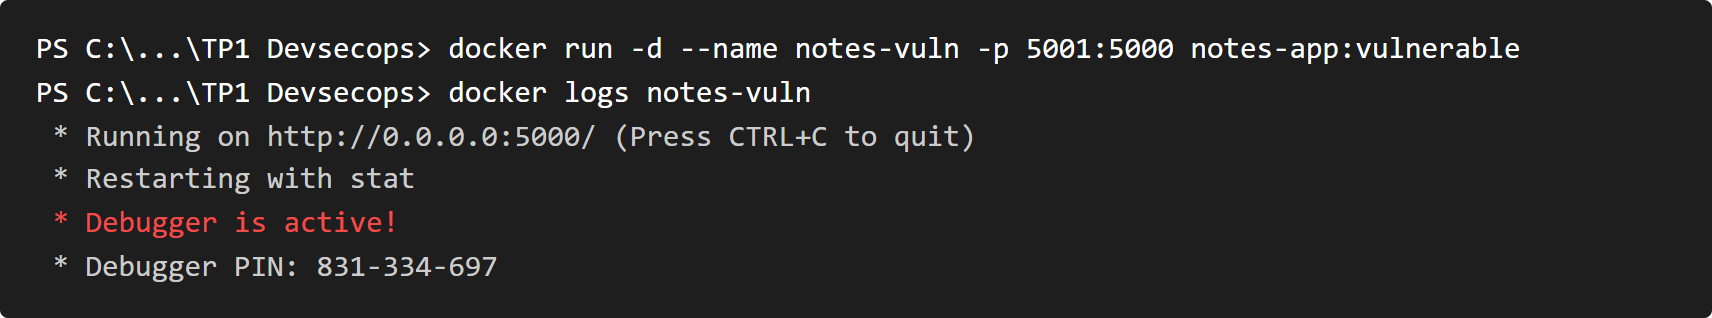
\includegraphics[width=0.92\textwidth]{t_vuln_logs.png}}
\caption{Lancement de l'image initiale : le débogueur Werkzeug est actif.}
\label{fig:vulnlogs}
\end{figure}


\subsection{Organisation du dépôt Git}
L'historique est découpé pour que chaque étape du TP soit visible et comparable :

\begin{table}[H]
\centering
\begin{tabularx}{\textwidth}{@{}lL@{}}
\toprule
\textbf{Commit / tag} & \textbf{Contenu} \\
\midrule
\code{v1.0-vulnerable} & Application initiale vulnérable \\
\code{SAST : correction\ldots} & Corrections des vulnérabilités signalées par Bandit + rapports Bandit \\
\code{v2.0-secure} & Mise à jour des dépendances, image Docker durcie, rapports SCA \\
Commits suivants & Script de scan, pipeline CI, rapport \\
\bottomrule
\end{tabularx}
\end{table}

% ---------------------------------------------------------------------------
\section{Partie II -- Analyse Statique (SAST) avec Bandit}
% ---------------------------------------------------------------------------
\subsection{Principe et lancement du scan}
Bandit parcourt l'arbre syntaxique (AST) de chaque fichier Python et applique des règles
(\code{B1xx} à \code{B7xx}). Chaque problème reçoit une \textbf{sévérité} (impact s'il est
exploitable) et un \textbf{niveau de confiance} (probabilité qu'il s'agisse d'un vrai problème).

\begin{lstlisting}[caption={Lancement de Bandit via Docker}]
docker run --rm -v "${PWD}:/src" -w /src --entrypoint bandit `
    ghcr.io/pycqa/bandit/bandit -r app -f html -o reports/sast/bandit-before.html
\end{lstlisting}

\subsection{Résultats initiaux}
Le premier scan signale \textbf{15 problèmes : 4 High, 7 Medium et 4 Low}.

\begin{table}[H]
\centering
\small
\begin{tabularx}{\textwidth}{@{}rllrL@{}}
\toprule
\textbf{\#} & \textbf{Règle} & \textbf{Sév. / Conf.} & \textbf{Ligne} & \textbf{Problème (CWE)} \\
\midrule
1  & B608 & Medium / Low    & 102 & Injection SQL dans \code{/login} (CWE-89) \\
2  & B608 & Medium / Low    & 152 & Injection SQL dans \code{/search} (CWE-89) \\
3  & B602 & \textbf{High} / High & 199 & Injection de commande OS, \code{shell=True} (CWE-78) \\
4  & B704 & Medium / High   & 157 & XSS réfléchi : \code{Markup()} sur la saisie (CWE-79) \\
5  & B301 & Medium / High   & 189 & Désérialisation \code{pickle} d'un cookie (CWE-502) \\
6  & B403 & Low / High      & 11  & Import du module \code{pickle} (CWE-502) \\
7  & B506 & Medium / High   & 166 & \code{yaml.load()} sur un fichier utilisateur (CWE-20) \\
8  & B324 & \textbf{High} / High & 47 & Mots de passe hachés en MD5 (CWE-327) \\
9  & B105 & Low / Medium    & 24  & \code{secret\_key} Flask en dur (CWE-259) \\
10 & B105 & Low / Medium    & 26  & Mot de passe administrateur en dur (CWE-259) \\
11 & B501 & \textbf{High} / High & 206 & \code{requests} avec \code{verify=False} (CWE-295) \\
12 & B113 & Medium / Low    & 206 & Requête HTTP sans timeout (CWE-400) \\
13 & B201 & \textbf{High} / Medium & 213 & \code{app.run(debug=True)} (CWE-94) \\
14 & B104 & Medium / Medium & 213 & Écoute sur \code{0.0.0.0} (CWE-605) \\
15 & B404 & Low / High      & 13  & Import du module \code{subprocess} (CWE-78) \\
\bottomrule
\end{tabularx}
\caption{Résultats Bandit sur la version initiale}
\end{table}

Le TP demande d'en corriger au moins deux. \textbf{Toutes les vulnérabilités High et Medium
ont été corrigées}, ainsi que les secrets en dur. Les deux premières sont détaillées
ci-dessous (Figures~\ref{fig:b608} et~\ref{fig:b602}).

\subsection{Vulnérabilité 1 -- Injection SQL (B608, CWE-89)}
\begin{lstlisting}[language=Python,caption={Code vulnérable de \code{/login}}]
query = "SELECT id, username FROM users WHERE username = '%s' AND password = '%s'" % (
    username,
    hash_password(password),
)
user = get_db().execute(query).fetchone()
\end{lstlisting}


\begin{figure}[H]
\centering
\fbox{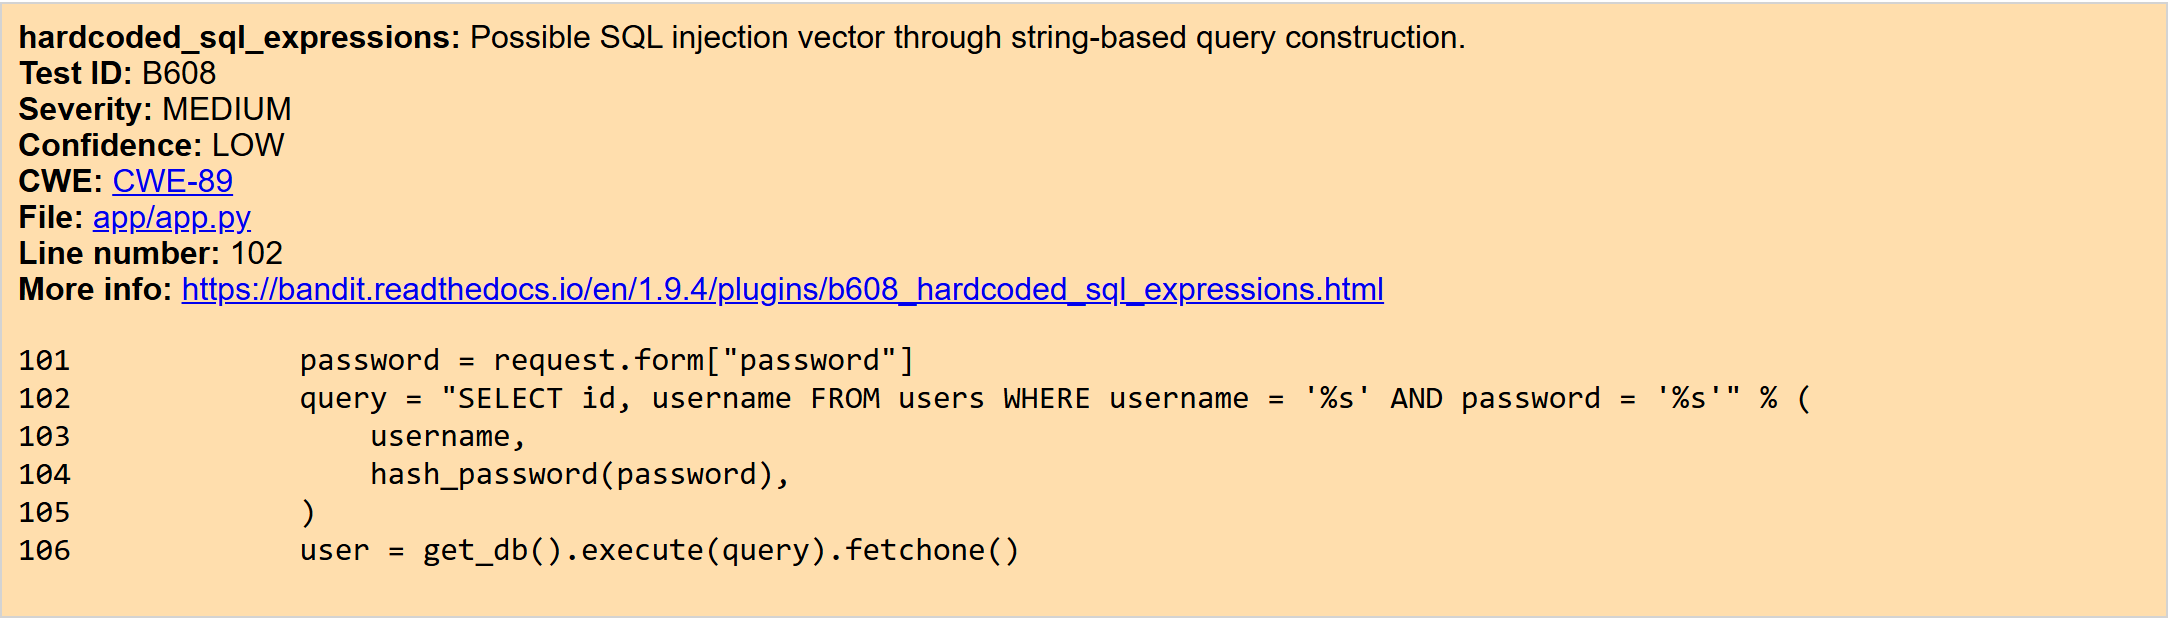
\includegraphics[width=0.92\textwidth]{r_bandit_b608.png}}
\caption{Rapport Bandit initial : injection SQL (B608) dans \code{/login}.}
\label{fig:b608}
\end{figure}

\paragraph{Pourquoi c'est dangereux.} La saisie de l'utilisateur est insérée directement dans le
texte de la requête SQL. Des caractères SQL (apostrophe, commentaire\ldots) peuvent alors
\textbf{modifier la structure de la requête} au lieu d'être traités comme des données. Sur
\code{/login}, un attaquant peut ainsi se connecter sous l'identité d'un autre utilisateur sans
connaître son mot de passe. Sur \code{/search}, il peut lire d'autres tables, par exemple les
hachés de mots de passe.

\paragraph{Correction : requêtes paramétrées.} La requête et les données sont transmises
séparément à SQLite. La saisie est toujours traitée comme une valeur, jamais comme du code.

\begin{lstlisting}[language=Python,caption={Code corrigé de \code{/login} et \code{/search}}]
# [SAST B608] Requete parametree : la saisie n'est jamais concatenee au SQL.
user = get_db().execute(
    "SELECT id, username, password FROM users WHERE username = ?",
    (request.form["username"],),
).fetchone()
if user and check_password_hash(user["password"], request.form["password"]):
    ...

notes = get_db().execute(
    "SELECT id, title, content FROM notes WHERE owner_id = ? AND title LIKE ?",
    (session["user_id"], "%" + q + "%"),
).fetchall()
\end{lstlisting}

\noindent\emph{Remarque :} Bandit attribue à B608 une confiance \emph{Low}. Il repère un motif
(une chaîne SQL formatée) sans pouvoir prouver que la variable provient de l'utilisateur. Ici,
c'est bien un \textbf{vrai positif}. L'analyse SAST demande donc toujours une vérification
humaine (triage).

\subsection{Vulnérabilité 2 -- Injection de commande OS (B602, CWE-78)}
\begin{lstlisting}[language=Python,caption={Code vulnérable de \code{/tools/ping}}]
host = request.args.get("host", "127.0.0.1")
output = subprocess.check_output("ping -c 1 " + host, shell=True, stderr=subprocess.STDOUT)
\end{lstlisting}


\begin{figure}[H]
\centering
\fbox{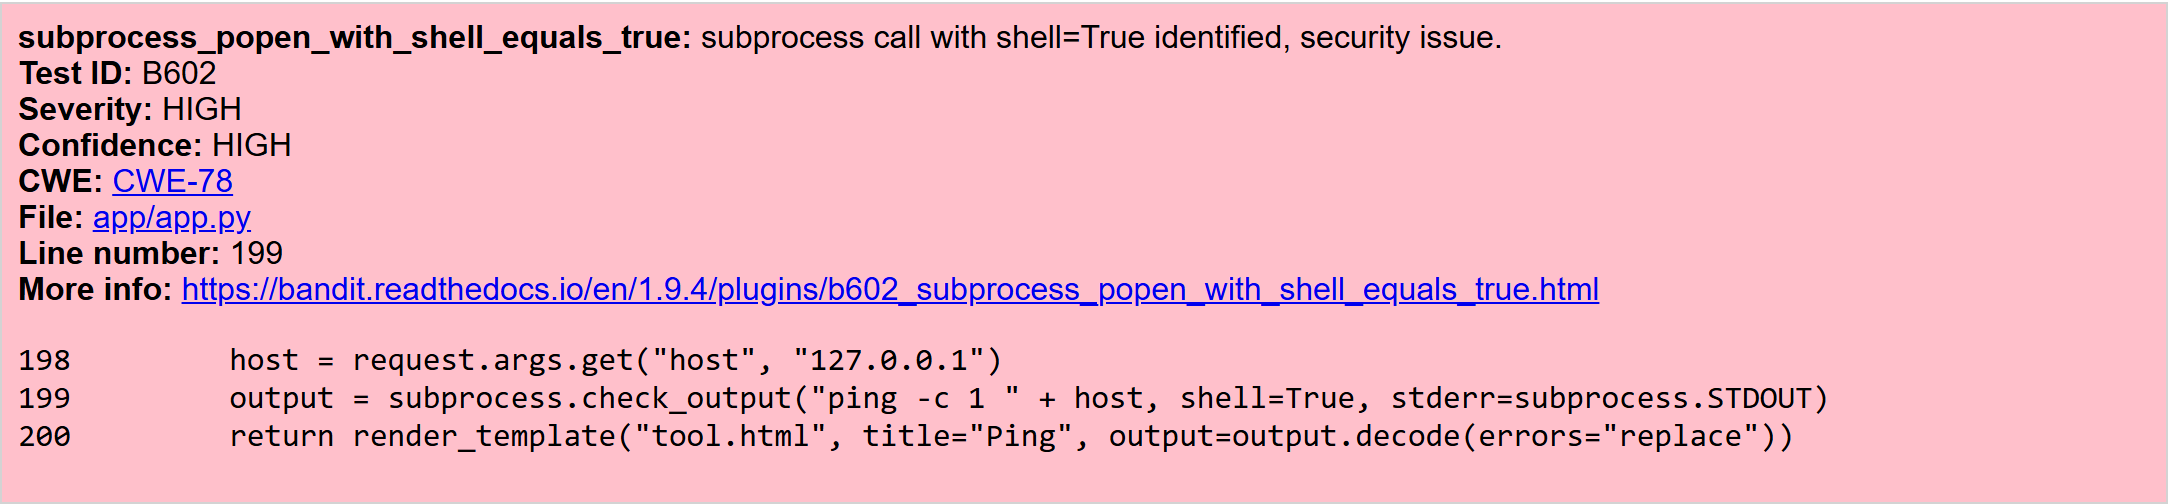
\includegraphics[width=0.92\textwidth]{r_bandit_b602.png}}
\caption{Rapport Bandit initial : injection de commande (B602, sévérité High).}
\label{fig:b602}
\end{figure}

\paragraph{Pourquoi c'est dangereux.} Avec \code{shell=True}, la chaîne est interprétée par
\code{/bin/sh}. Les métacaractères du shell (\code{;}, \code{\&\&}, \code{|}\ldots) présents dans
\code{host} permettent d'enchaîner \textbf{n'importe quelle commande} sur le serveur. Dans
l'image initiale, le processus tourne en \textbf{root} et la route n'exige aucune authentification :
c'est une exécution de code à distance (RCE).

\paragraph{Correction : validation stricte et suppression du shell.} La saisie est d'abord validée comme adresse IP, puis la commande est lancée sans shell :
\begin{lstlisting}[language=Python,caption={Code corrigé de \code{/tools/ping}}]
@app.route("/tools/ping")
@login_required
def ping():
    # [SAST B602] Validation stricte de l'entree (adresse IP uniquement) et
    # appel sans shell, avec une liste d'arguments et un chemin absolu.
    try:
        ip = ipaddress.ip_address(request.args.get("host", "127.0.0.1"))
    except ValueError:
        abort(400, "Adresse IP invalide")
    result = subprocess.run(
        ["/bin/ping", "-c", "1", str(ip)], capture_output=True, timeout=5, check=False
    )
\end{lstlisting}

\begin{enumerate}[leftmargin=*]
  \item \textbf{Liste blanche} : seule une adresse IPv4/IPv6 valide est acceptée ; tout le reste
        renvoie une erreur 400 (Figure~\ref{fig:ping400}).
  \item \textbf{Pas de shell} : la commande est une liste d'arguments, aucun métacaractère n'est
        interprété.
  \item \textbf{Chemin absolu} \code{/bin/ping} (évite un détournement par le \code{PATH}),
        \textbf{timeout}, \textbf{authentification} obligatoire et, dans l'image, utilisateur
        \textbf{non-root}.
\end{enumerate}


\begin{figure}[H]
\centering
\fbox{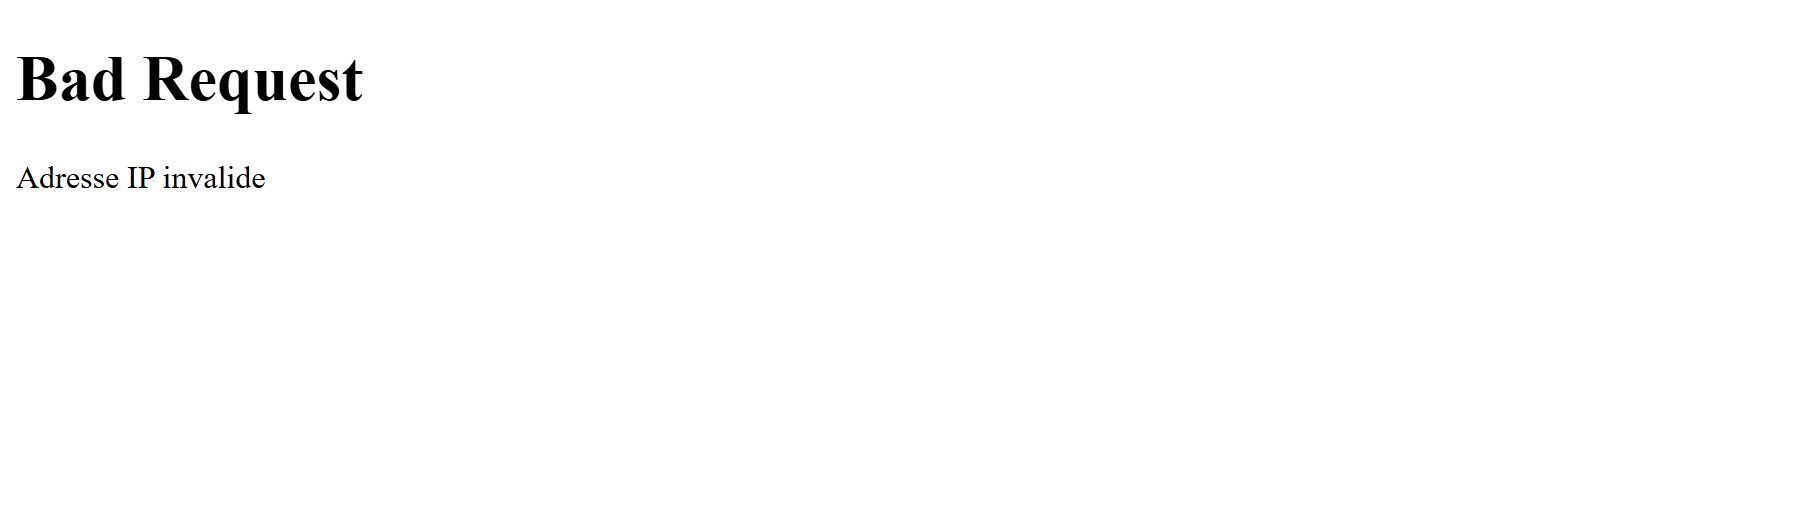
\includegraphics[width=0.7\textwidth,trim=0 290 0 0,clip]{a_secure_ping_400.png}}
\caption{Outil ping avec une valeur qui n'est pas une adresse IP : requête refusée (HTTP 400).}
\label{fig:ping400}
\end{figure}

\subsection{Autres vulnérabilités corrigées}
\begin{table}[H]
\centering
\small
\begin{tabularx}{\textwidth}{@{}lLL@{}}
\toprule
\textbf{Règle} & \textbf{Risque} & \textbf{Correction apportée} \\
\midrule
B704 (XSS) & \code{Markup()} désactive l'échappement : du JavaScript peut s'exécuter dans le navigateur de la victime & Suppression de \code{Markup()} ; échappement automatique de Jinja2 (Figure~\ref{fig:search}) ; en-tête CSP \\
B301 / B403 (pickle) & Désérialiser un cookie contrôlé par le client revient à exécuter du code arbitraire & Préférence stockée dans la session Flask (JSON signé HMAC) + liste blanche des valeurs \\
B506 (\code{yaml.load}) & Instanciation d'objets Python arbitraires ; combiné à PyYAML 5.3 : RCE (\S\ref{sec:pyyaml}) & \code{yaml.safe\_load()} + validation de la structure + taille d'upload limitée à 1~Mo \\
B324 (MD5) & Hachés cassables en quelques secondes en cas de fuite de la base & \code{generate\_password\_hash()} de Werkzeug (scrypt, sel aléatoire) \\
B105 (secrets en dur) & \code{secret\_key} connue : forge de sessions ; secrets visibles dans l'historique Git & Variables d'environnement \code{SECRET\_KEY} et \code{ADMIN\_PASSWORD} ; clé aléatoire par défaut \\
B501 / B113 & Interception TLS (MITM) ; blocage des workers (DoS) ; SSRF vers le réseau interne & \code{verify=True}, \code{timeout=5}, pas de redirection, seules les URL publiques en http(s) sont acceptées \\
B201 / B104 & Débogueur Werkzeug exposé, qui permet d'exécuter du Python & \code{debug} piloté par \code{FLASK\_DEBUG}, écoute sur \code{127.0.0.1}, \textbf{gunicorn} en production \\
\bottomrule
\end{tabularx}
\caption{Synthèse des autres corrections SAST}
\end{table}


\begin{figure}[H]
\centering
\fbox{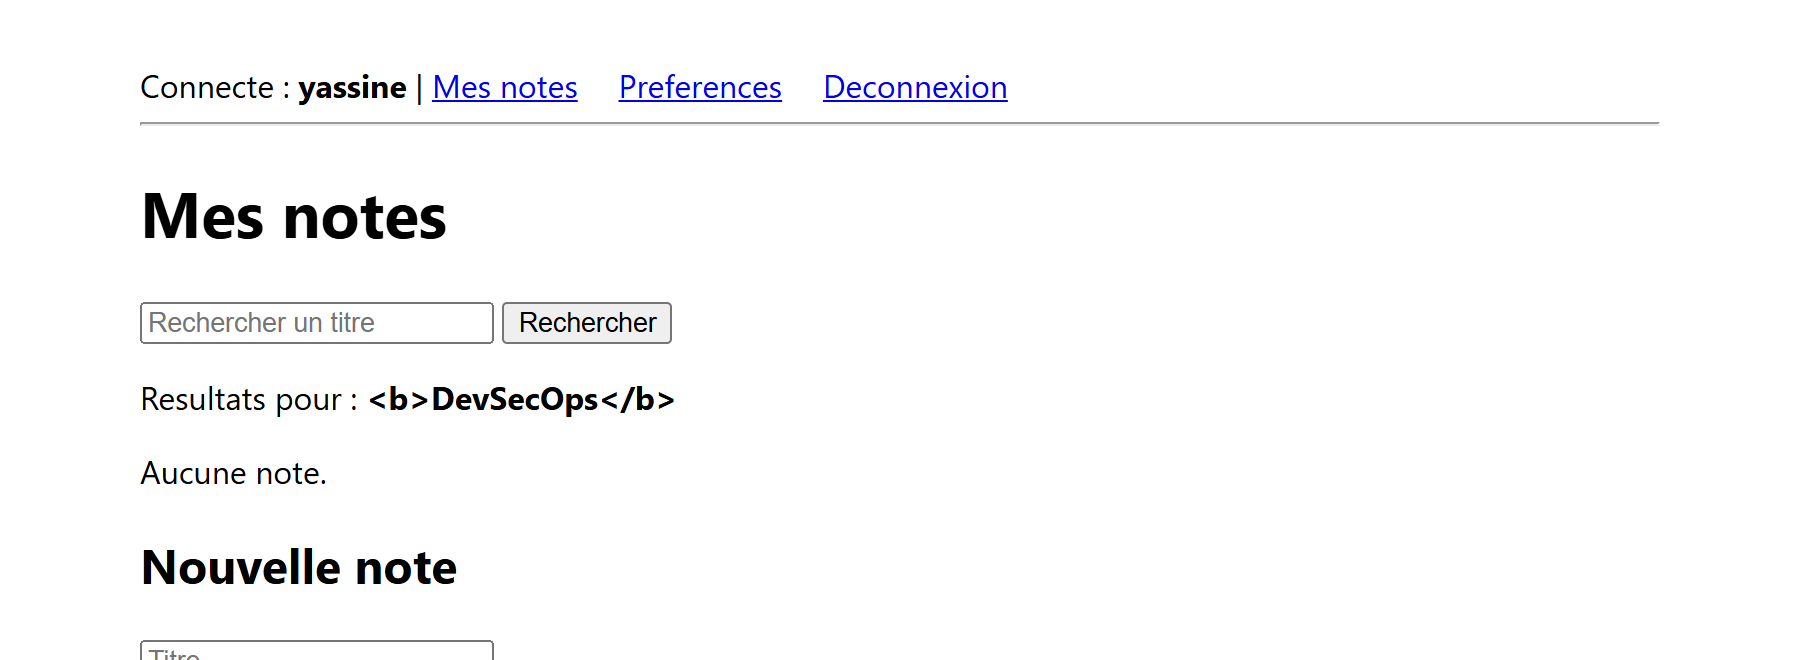
\includegraphics[width=0.7\textwidth]{a_secure_search.png}}
\caption{Recherche contenant du HTML : la saisie est affichée échappée (correction B704).}
\label{fig:search}
\end{figure}

\subsection{Résultats après correction}
\begin{table}[H]
\centering
\begin{tabular}{@{}lcc@{}}
\toprule
\textbf{Sévérité} & \textbf{Avant} & \textbf{Après} \\
\midrule
High   & 4  & \textbf{0} \\
Medium & 7  & \textbf{0} \\
Low    & 4  & 2 \\
\midrule
Total  & 15 & 2 \\
\bottomrule
\end{tabular}
\caption{Bandit avant / après correction}
\end{table}

Les \textbf{deux problèmes Low restants} (Figure~\ref{fig:banditafter}) ont été analysés et
\textbf{acceptés} :
\begin{itemize}
  \item \textbf{B404} (import de \code{subprocess}) : avertissement générique, le module est
        nécessaire à la fonctionnalité ping.
  \item \textbf{B603} (\code{subprocess} sans shell) : Bandit rappelle de vérifier les entrées.
        C'est fait : pas de shell, chemin absolu, argument validé par \code{ipaddress}.
\end{itemize}

\begin{figure}[H]
\centering
\fbox{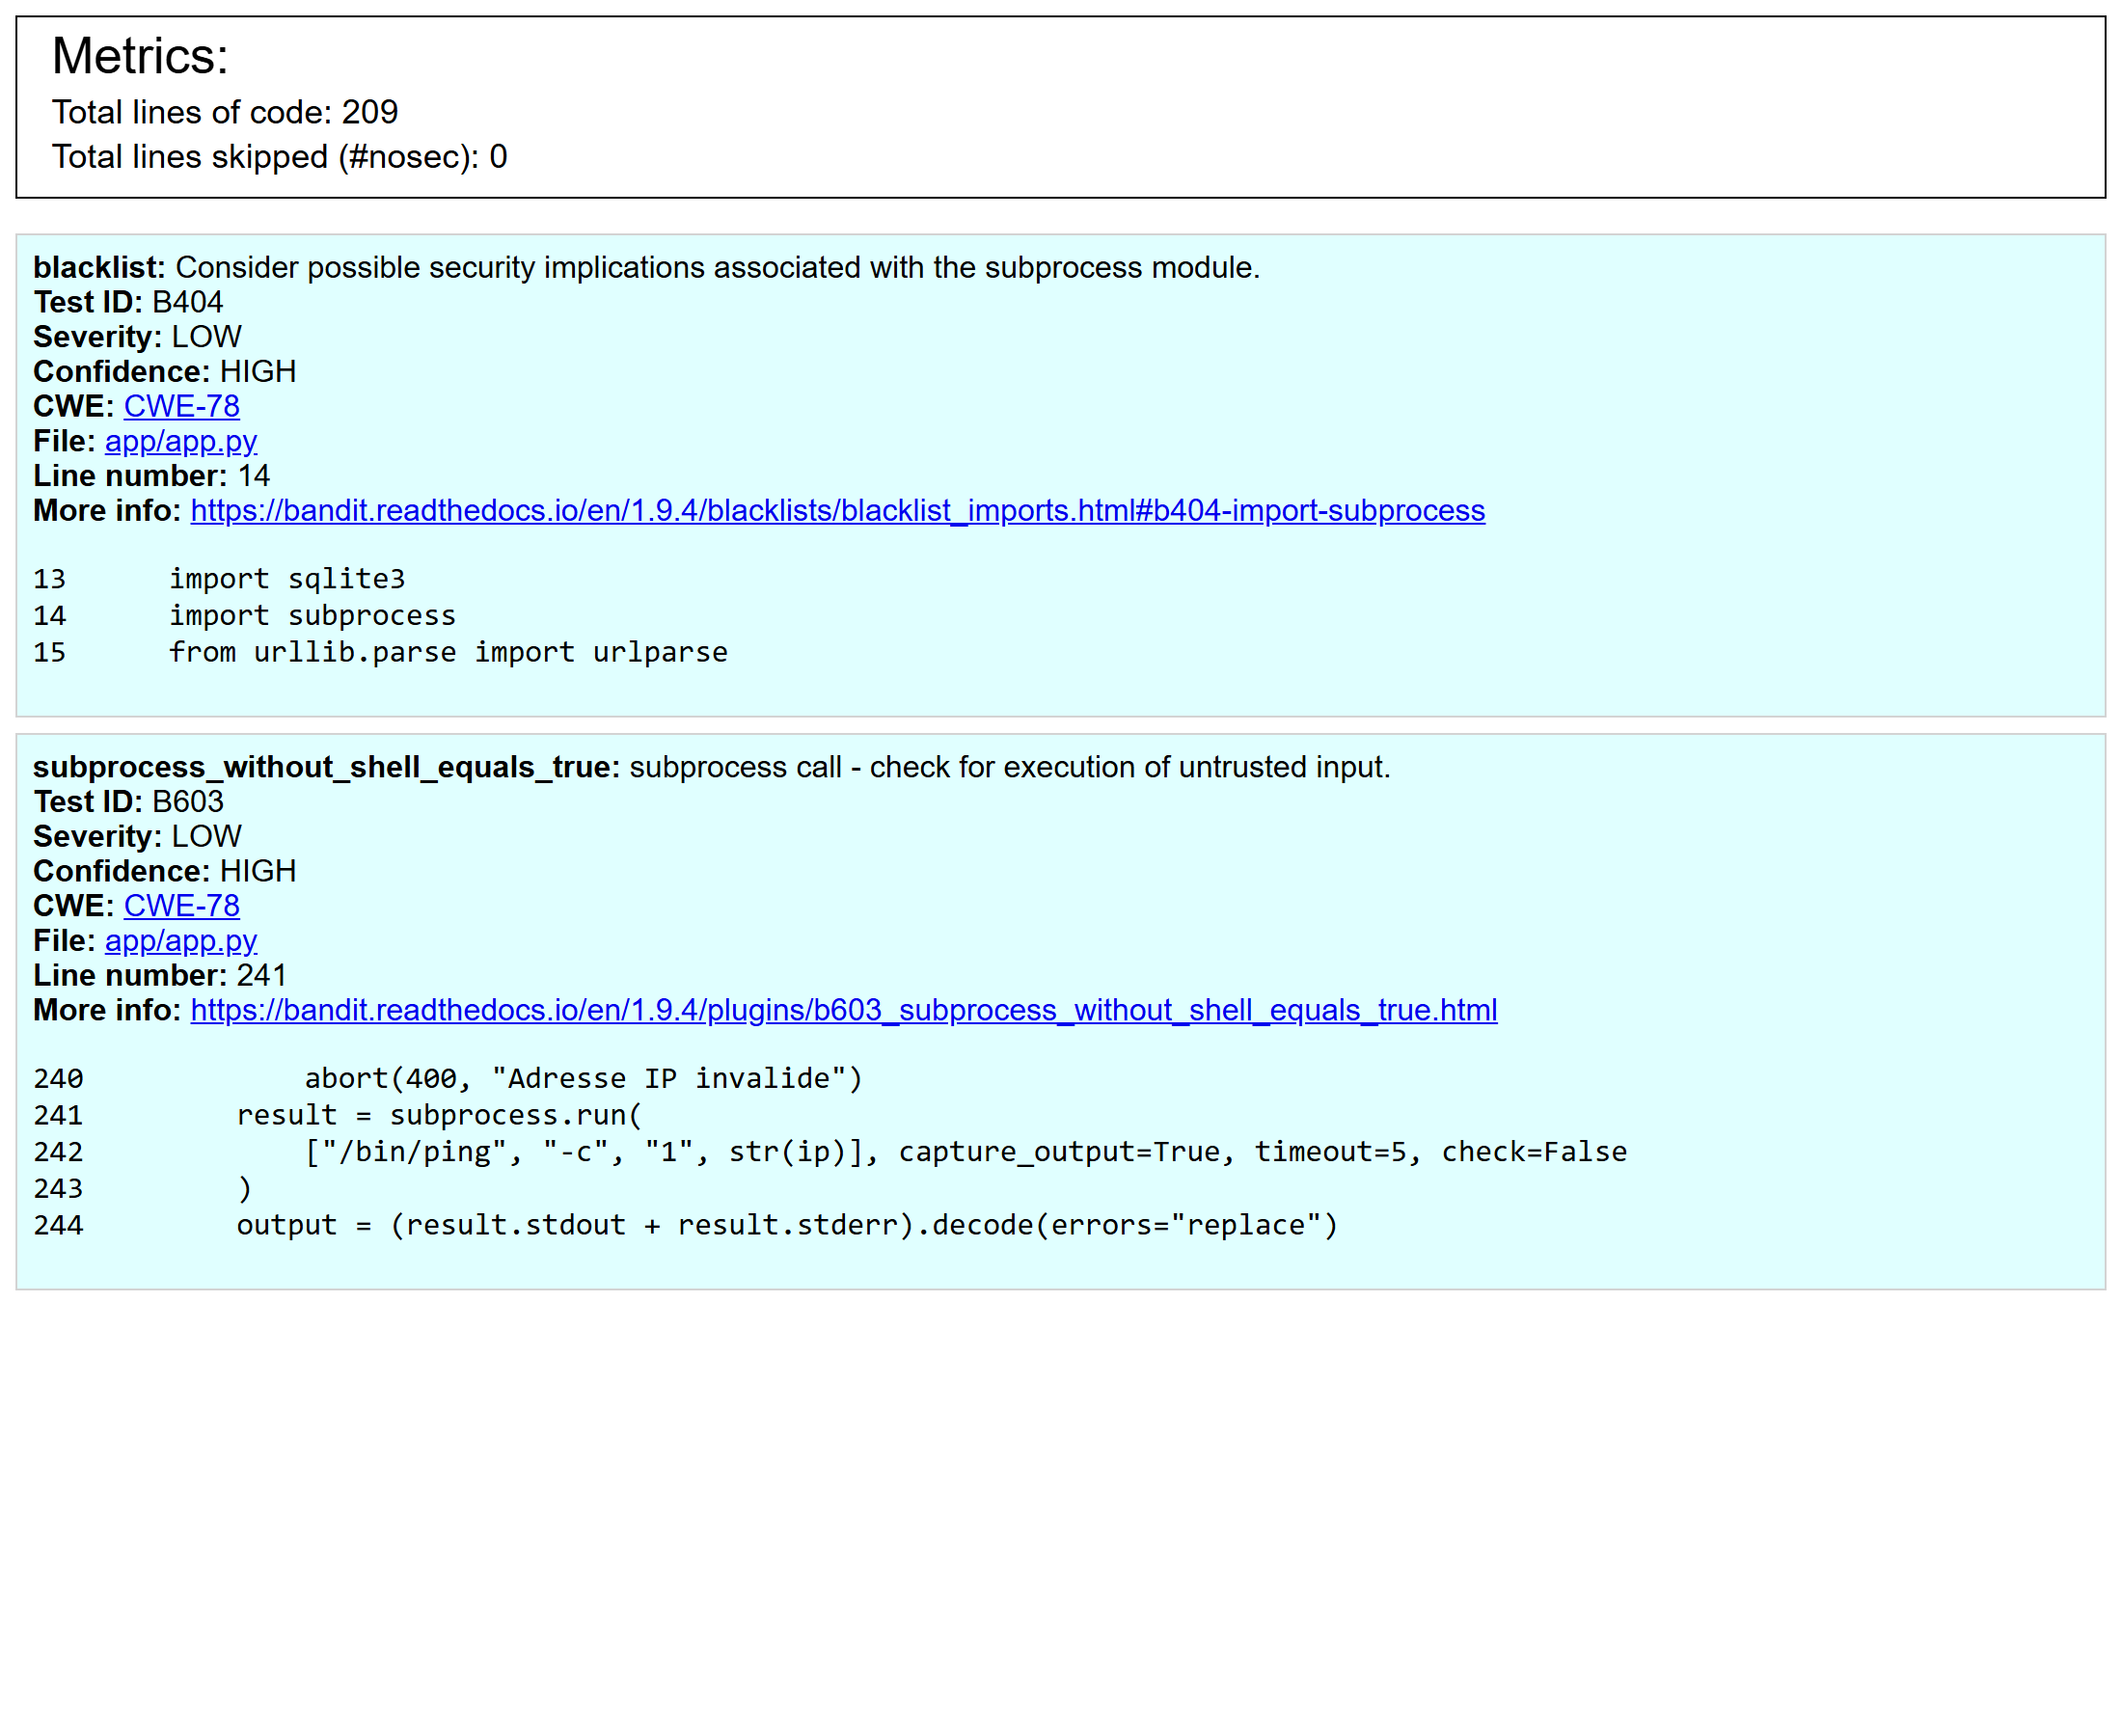
\includegraphics[width=0.85\textwidth,trim=0 430 0 0,clip]{r_bandit-after.png}}
\caption{Rapport Bandit après correction : seules restent les deux alertes Low B404 et B603.}
\label{fig:banditafter}
\end{figure}

Ces lignes n'ont volontairement \textbf{pas} été masquées par \code{\# nosec}, par souci de
transparence. En CI, le seuil de blocage est fixé à \emph{Medium}.

\subsection{Limites observées du SAST}
\begin{itemize}
  \item \textbf{Faux positifs possibles} : les règles à confiance \emph{Low} demandent une
        confirmation humaine.
  \item \textbf{Faux négatifs} : Bandit ne raisonne pas sur la logique applicative. Il n'a pas
        détecté la SSRF de \code{/tools/fetch}, l'absence d'authentification des outils réseau ni
        l'absence de protection CSRF. Ces points ont été trouvés à la relecture.
  \item Bandit n'analyse ni les templates, ni le Dockerfile, ni les dépendances : c'est le rôle de la SCA.
\end{itemize}

% ---------------------------------------------------------------------------
\section{Partie III -- Analyse des Dépendances (SCA)}
% ---------------------------------------------------------------------------
\subsection{Outils et commandes}
\textbf{OWASP Dependency-Check} identifie chaque composant, lui associe un identifiant
\textbf{CPE} puis recherche les \textbf{CVE} correspondantes dans la base \textbf{NVD} du NIST.

\begin{lstlisting}[caption={Lancement d'OWASP Dependency-Check}]
docker run --rm -v "${PWD}:/src" -v dc-data:/usr/share/dependency-check/data `
  owasp/dependency-check:latest `
  --project "TP1 Notes App" --scan /src --exclude "**/reports/**" --exclude "**/.git/**" `
  --enableExperimental --disableOssIndex `
  --nvdDatafeed "https://dependency-check.github.io/DependencyCheck_Builder/nvd_cache/" `
  --format HTML --format JSON --out /src/reports/sca
\end{lstlisting}

\begin{itemize}
  \item \code{-{}-enableExperimental} : l'analyseur de \code{requirements.txt} est expérimental.
        Sans cette option, aucune dépendance Python n'est détectée.
  \item \code{-{}-nvdDatafeed} : sans clé d'API NVD, le téléchargement par l'API est très limité en
        débit. On utilise le miroir du projet Dependency-Check (environ 100~s au premier lancement),
        conservé ensuite dans le volume \code{dc-data}.
  \item \code{-{}-disableOssIndex} : l'analyseur Sonatype OSS Index demande désormais un jeton personnel.
\end{itemize}

\textbf{pip-audit} (outil de la PyPA) sert de \textbf{contre-vérification}. Il identifie les
paquets par leur nom PyPI exact et interroge la base OSV / PyPI Advisory :

\begin{lstlisting}[caption={Lancement de pip-audit}]
docker run --rm -v "${PWD}:/src" -w /src python:3.13-slim sh -c `
  "pip install -q pip-audit && pip-audit -r requirements.txt --no-deps --disable-pip"
\end{lstlisting}

\subsection{Résultats initiaux}
\begin{table}[H]
\centering
\begin{tabularx}{\textwidth}{@{}lLl@{}}
\toprule
\textbf{Analyse} & \textbf{Cible} & \textbf{Résultat} \\
\midrule
Dependency-Check & \code{requirements.txt} & \textbf{4 CVE} (3 Critical, 1 High) \\
Dependency-Check & Paquets installés dans l'image Docker & \textbf{44 alertes} (7 Critical, 12 High) \\
pip-audit & \code{requirements.txt} & \textbf{47 vulnérabilités} dans 9 paquets \\
\bottomrule
\end{tabularx}
\caption{Résultats SCA sur la version initiale (Figures~\ref{fig:dcbefore} et~\ref{fig:dcimage})}
\end{table}


\begin{figure}[H]
\centering
\fbox{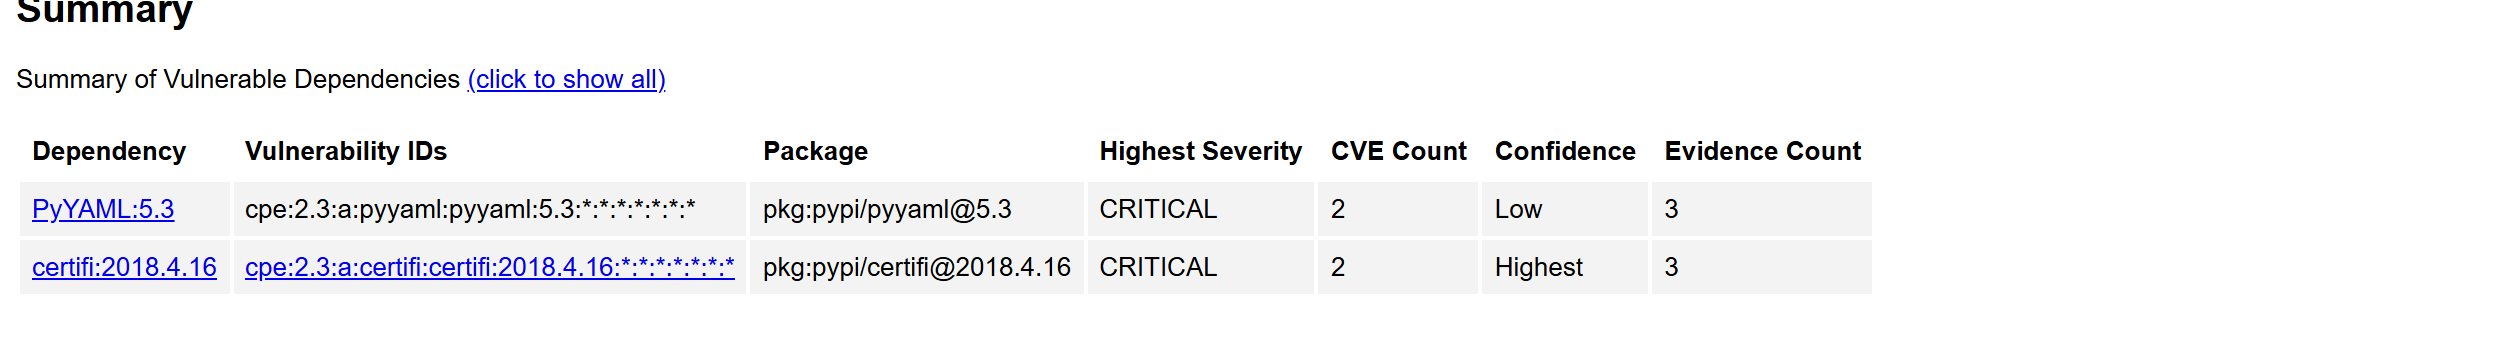
\includegraphics[width=0.85\textwidth,trim=0 0 600 0,clip]{r_dependency-check-before.png}}
\caption{OWASP Dependency-Check sur \code{requirements.txt} (version initiale).}
\label{fig:dcbefore}
\end{figure}

\begin{figure}[H]
\centering
\fbox{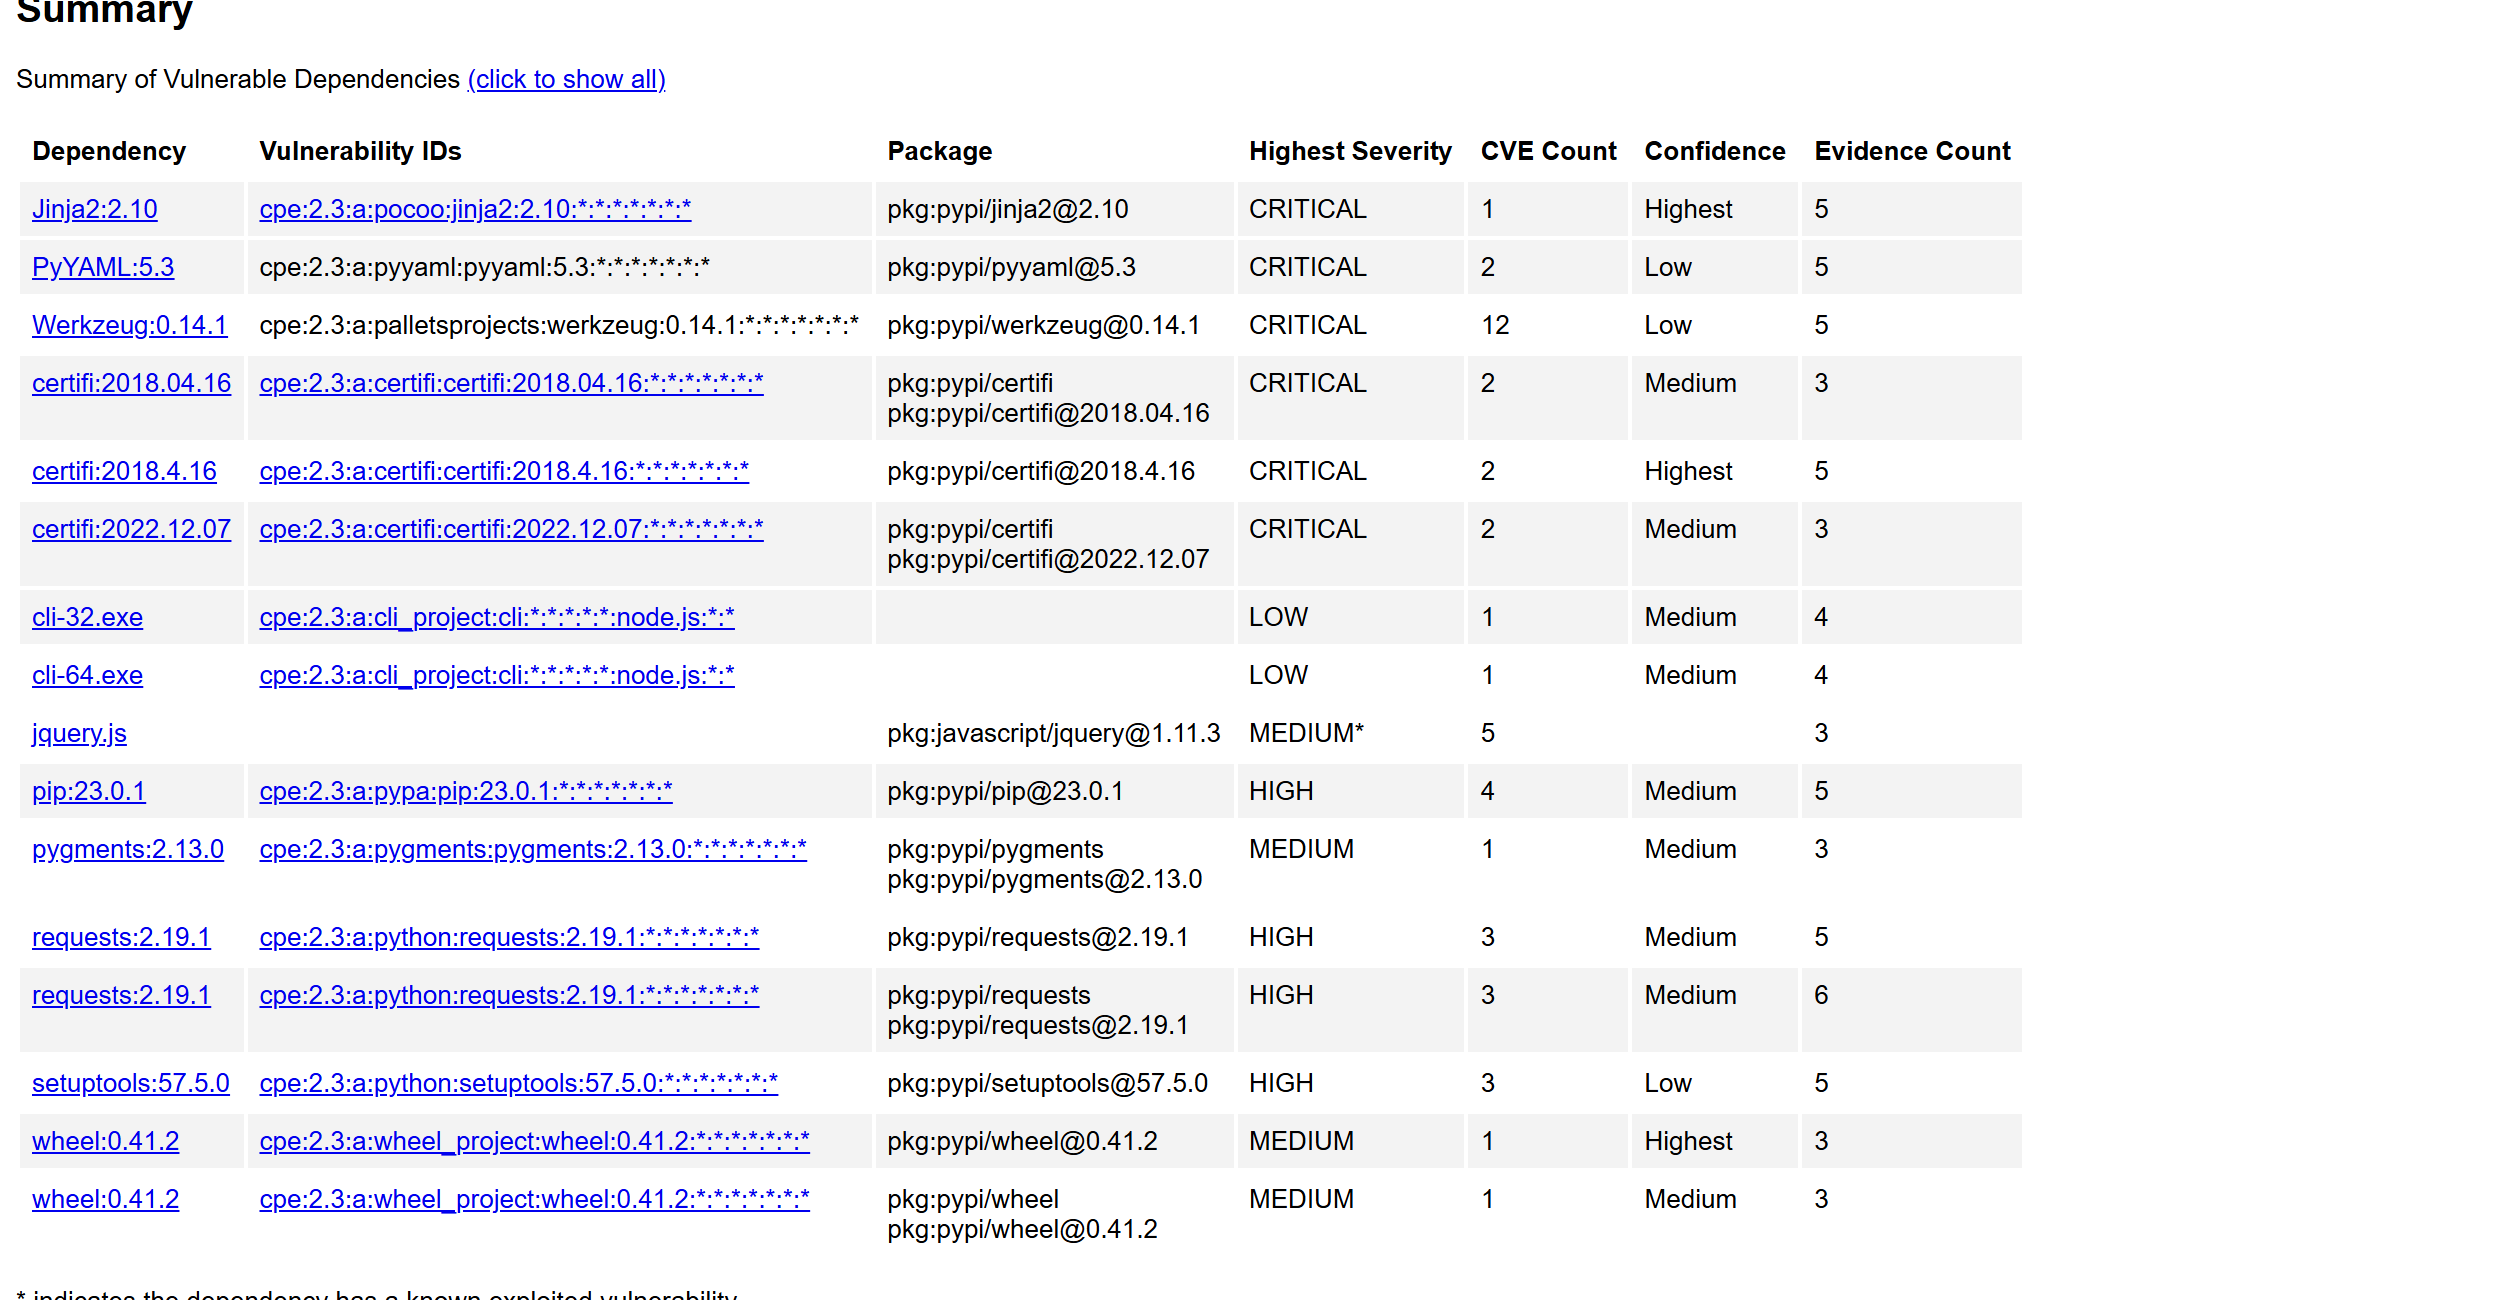
\includegraphics[width=0.95\textwidth,trim=0 0 440 0,clip]{r_dependency-check-image-before.png}}
\caption{OWASP Dependency-Check sur les paquets installés dans l'image initiale.}
\label{fig:dcimage}
\end{figure}


\begin{table}[H]
\centering
\small
\begin{tabularx}{\textwidth}{@{}llcLl@{}}
\toprule
\textbf{Paquet} & \textbf{Version} & \textbf{Nb} & \textbf{Vulnérabilité la plus marquante (CVSS NVD)} & \textbf{Retenue} \\
\midrule
PyYAML   & 5.3       & 2  & CVE-2020-1747 / CVE-2020-14343 : \textbf{9.8 Critical}, exécution de code & \textbf{6.0.3} \\
Werkzeug & 0.14.1    & 12 & CVE-2022-29361 : 9.8 (\emph{request smuggling}) ; CVE-2019-14806 : 7.5 (PIN du débogueur) & 3.1.9 \\
certifi  & 2018.4.16 & 2  & CVE-2023-37920 : 9.8 (autorités racines non fiables) & 2026.7.22 \\
requests & 2.19.1    & 5  & CVE-2018-18074 : 7.5 (fuite de l'en-tête \code{Authorization}) & 2.34.2 \\
urllib3  & 1.23      & 12 & CVE-2023-43804 (fuite de cookies lors de redirections) & 2.8.0 \\
Jinja2   & 2.10      & 6  & CVE-2019-10906, CVE-2025-27516 (évasions du \emph{sandbox}) & 3.1.6 \\
Flask    & 0.12.2    & 4  & CVE-2018-1000656 (DoS), CVE-2023-30861 (cookie de session mis en cache) & 3.1.3 \\
gunicorn & 19.9.0    & 2  & CVE-2024-1135 (\emph{HTTP request smuggling}) & 26.2.0 \\
idna     & 2.7       & 2  & CVE-2024-3651 (DoS) & 3.20 \\
\bottomrule
\end{tabularx}
\caption{Synthèse par paquet (détail des 47 vulnérabilités en annexe, page~\pageref{sec:cve})}
\end{table}

\subsection{Dépendance vulnérable choisie : PyYAML 5.3 \texorpdfstring{$\rightarrow$}{->} 6.0.3}\label{sec:pyyaml}
\paragraph{Les vulnérabilités.}
\begin{itemize}
  \item \textbf{CVE-2020-1747} (CVSS 9.8, Critical) : dans PyYAML $<$ 5.3.1, le chargement d'un
        YAML non fiable avec \code{full\_load()} ou le \code{FullLoader} permet une
        \textbf{exécution de code arbitraire}, en abusant du constructeur \code{python/object/new}.
  \item \textbf{CVE-2020-14343} (CVSS 9.8, Critical) : le correctif de la version 5.3.1 était
        \textbf{incomplet}. La même attaque restait possible jusqu'à la version 5.4.
\end{itemize}

\paragraph{Pourquoi cette mise à jour est nécessaire.}
\begin{enumerate}[leftmargin=*]
  \item \textbf{La faille était directement exploitable} : la route \code{/import} passait un
        fichier envoyé par l'utilisateur à \code{yaml.load()} sans \code{Loader}. Avec PyYAML 5.x,
        ce cas utilise par défaut le \code{FullLoader}, précisément celui des deux CVE. C'est une
        exécution de code à distance de gravité maximale (exploitable à distance, sans privilège,
        sans interaction).
  \item \textbf{Corriger le code ne suffit pas} : c'est une défense en profondeur. Si un
        \code{full\_load()} est réintroduit plus tard, ou si une autre bibliothèque utilise
        PyYAML, la version corrigée protège toujours.
  \item \textbf{PyYAML 6 est plus sûr par conception} : \code{yaml.load()} sans \code{Loader}
        explicite lève désormais une erreur. Le piège à l'origine de la faille n'existe plus.
  \item \textbf{Choix de la version} : la version minimale corrigée est la 5.4. Nous avons retenu
        la dernière version stable, 6.0.3, compatible Python 3.13 et sans vulnérabilité connue
        selon les deux outils.
\end{enumerate}

\noindent Ce cas illustre la \textbf{complémentarité SAST / SCA} : Bandit signale le mauvais
\emph{usage} de la bibliothèque (B506), Dependency-Check signale sa \emph{version} vulnérable.

\subsection{Autres mises à jour}
\begin{table}[H]
\centering
\small
\begin{tabularx}{\textwidth}{@{}lL@{}}
\toprule
\textbf{Paquet} & \textbf{Justification principale} \\
\midrule
Werkzeug 3.1.9 & Les CVE du débogueur (CVE-2019-14806 : PIN prévisible \emph{dans Docker} ; CVE-2024-34069) aggravaient directement B201 (\code{debug=True}). S'y ajoutent des DoS sur les formulaires multipart. \\
Flask 3.1.3 & DoS par JSON mal encodé, fuite possible du cookie de session via un proxy cache. \\
requests 2.34.2 / urllib3 2.8.0 & Fuites d'en-têtes \code{Authorization} / \code{Cookie} lors de redirections. CVE-2024-35195 : une première requête en \code{verify=False} pouvait désactiver la vérification TLS pour toute la \code{Session}, en lien direct avec B501. \\
certifi 2026.7.22 & Le magasin de 2018 contenait des autorités retirées par Mozilla (TrustCor, e-Tugra). La vérification TLS ne vaut que si la liste des autorités de confiance est à jour. \\
gunicorn 26.2.0 & \emph{Request smuggling} via des en-têtes \code{Transfer-Encoding} contradictoires (CVE-2024-1135, CVE-2024-6827). \\
Jinja2 3.1.6 & Évasions du \emph{sandbox}, ReDoS, injection d'attributs via \code{xmlattr}. \\
\bottomrule
\end{tabularx}
\end{table}

\noindent Toutes les versions restent \textbf{figées} (\code{==}) dans \code{requirements.txt},
dépendances transitives comprises. Le build est ainsi reproductible et la SCA porte exactement
sur ce qui est déployé.

\subsection{Durcissement de l'image Docker}
Le scan de l'image a aussi révélé des vulnérabilités dans les outils de la base Python 3.7
(\code{pip}, \code{setuptools}, \code{wheel}). Python 3.7 n'est plus maintenu depuis juin 2023.

\begin{lstlisting}[caption={Dockerfile final (version \code{v2.0-secure})}]
FROM python:3.13-slim
ENV PYTHONDONTWRITEBYTECODE=1 PYTHONUNBUFFERED=1 PIP_NO_CACHE_DIR=1 \
    DATABASE_PATH=/app/data/notes.db
WORKDIR /app
RUN apt-get update && apt-get install -y --no-install-recommends iputils-ping \
 && rm -rf /var/lib/apt/lists/* && useradd --create-home --uid 10001 appuser
COPY requirements.txt .
RUN pip install --upgrade pip && pip install -r requirements.txt
COPY app/ ./app/
RUN mkdir -p /app/data && chown appuser:appuser /app/data
USER appuser
EXPOSE 5000
HEALTHCHECK --interval=30s --timeout=3s --start-period=5s CMD python -c "..." || exit 1
CMD ["gunicorn", "--bind", "0.0.0.0:5000", "--workers", "2", "--preload", "--chdir", "app", "app:app"]
\end{lstlisting}

\begin{table}[H]
\centering
\begin{tabularx}{\textwidth}{@{}LL@{}}
\toprule
\textbf{Avant} & \textbf{Après} \\
\midrule
Python 3.7 (fin de vie) & Python 3.13 (maintenu, sans \code{setuptools} ni \code{wheel}) \\
Conteneur exécuté en \textbf{root} & Utilisateur \code{appuser} (uid 10001) \\
Serveur de développement + débogueur & \textbf{gunicorn}, serveur WSGI de production \\
\code{COPY . .} (tout le dépôt) & Copie de \code{requirements.txt} et \code{app/} seulement \\
Aucune supervision & \code{HEALTHCHECK} \\
\bottomrule
\end{tabularx}
\end{table}

\subsection{Résultats après mise à jour}
\begin{table}[H]
\centering
\begin{tabular}{@{}lcc@{}}
\toprule
\textbf{Analyse} & \textbf{Avant} & \textbf{Après} \\
\midrule
Dependency-Check -- \code{requirements.txt} & 4 CVE (3 Critical) & \textbf{0} \\
Dependency-Check -- image Docker & 44 alertes (7 Critical) & \textbf{0} \\
pip-audit & 47 vulnérabilités / 9 paquets & \textbf{0} \\
\bottomrule
\end{tabular}
\caption{SCA avant / après mise à jour (Figure~\ref{fig:dcafter})}
\end{table}


\begin{figure}[H]
\centering
\fbox{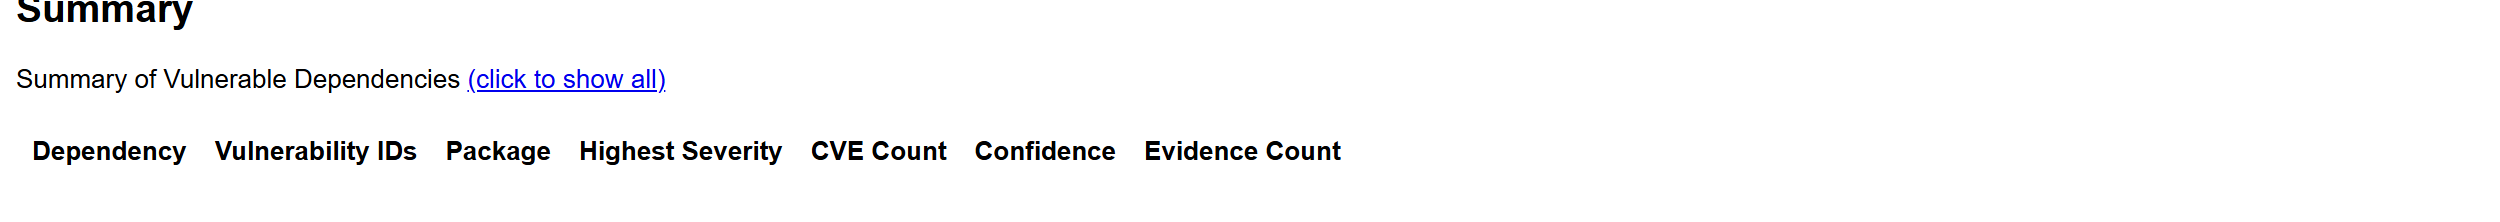
\includegraphics[width=0.6\textwidth,trim=0 0 1100 0,clip]{r_dependency-check-after.png}}
\caption{OWASP Dependency-Check après mise à jour : aucune dépendance vulnérable.}
\label{fig:dcafter}
\end{figure}

\subsection{Comparaison des outils SCA}
\begin{itemize}
  \item \textbf{Dependency-Check sur \code{requirements.txt}} ne trouve que 4 CVE sur 2 paquets,
        contre 47 sur 9 pour pip-audit. Il doit deviner l'identifiant CPE du paquet, qui contient
        un éditeur (\og palletsprojects \fg{} pour Werkzeug), or une ligne \code{Werkzeug==0.14.1} ne donne
        qu'un nom et une version : ce sont des \textbf{faux négatifs}.
  \item \textbf{Sur l'image}, les métadonnées des paquets installés (\code{*.dist-info}) donnent
        plus d'indices : Werkzeug (12 CVE), requests, Jinja2\ldots{} sont détectés. Flask, urllib3
        et gunicorn restent manqués. Le rapport contient aussi des \textbf{doublons} (copies
        embarquées dans \code{pip}), des \textbf{faux positifs} (\code{cli-32.exe} de setuptools
        associé à un paquet npm) et un \code{jquery 1.11.3} embarqué dans le débogueur de Werkzeug.
  \item \textbf{pip-audit} identifie les paquets par leur nom PyPI exact et indique directement la
        version corrigée : il est plus précis pour Python, mais ne voit pas l'image.
\end{itemize}
\textbf{Conclusion :} aucun outil SCA n'est exhaustif. Il faut croiser les sources (NVD, OSV),
analyser aussi l'artefact livré (l'image) et trier les résultats.

% ---------------------------------------------------------------------------
\section{Partie IV -- Démonstration et Évaluation}
% ---------------------------------------------------------------------------
\subsection{Scénario de démonstration}
Le script \code{scripts/scan.ps1} extrait une version Git (\code{git archive}, sans modifier la
copie de travail), puis lance Bandit, pip-audit et Dependency-Check dans Docker. Il affiche une
synthèse et enregistre les rapports.

\begin{enumerate}[leftmargin=*]
  \item \textbf{Vulnérabilités initiales} : \code{.\textbackslash scripts\textbackslash scan.ps1 -Ref v1.0-vulnerable}
        (Figure~\ref{fig:scanbefore}), puis ouverture des rapports HTML de Bandit et de Dependency-Check.
  \item \textbf{Correctifs} : \code{git diff v1.0-vulnerable v2.0-secure} \code{-{}- app/app.py requirements.txt Dockerfile}.
  \item \textbf{Les scanners ne signalent plus les problèmes corrigés} :
        \code{.\textbackslash scripts\textbackslash scan.ps1 -Ref v2.0-secure} (Figure~\ref{fig:scanafter}).
  \item \textbf{L'application corrigée fonctionne} (Figures~\ref{fig:notes} et~\ref{fig:pingok}) :
        conteneur \code{healthy} exécuté par \code{appuser}, saisies invalides refusées (HTTP 400).
\end{enumerate}


\begin{figure}[H]
\centering
\fbox{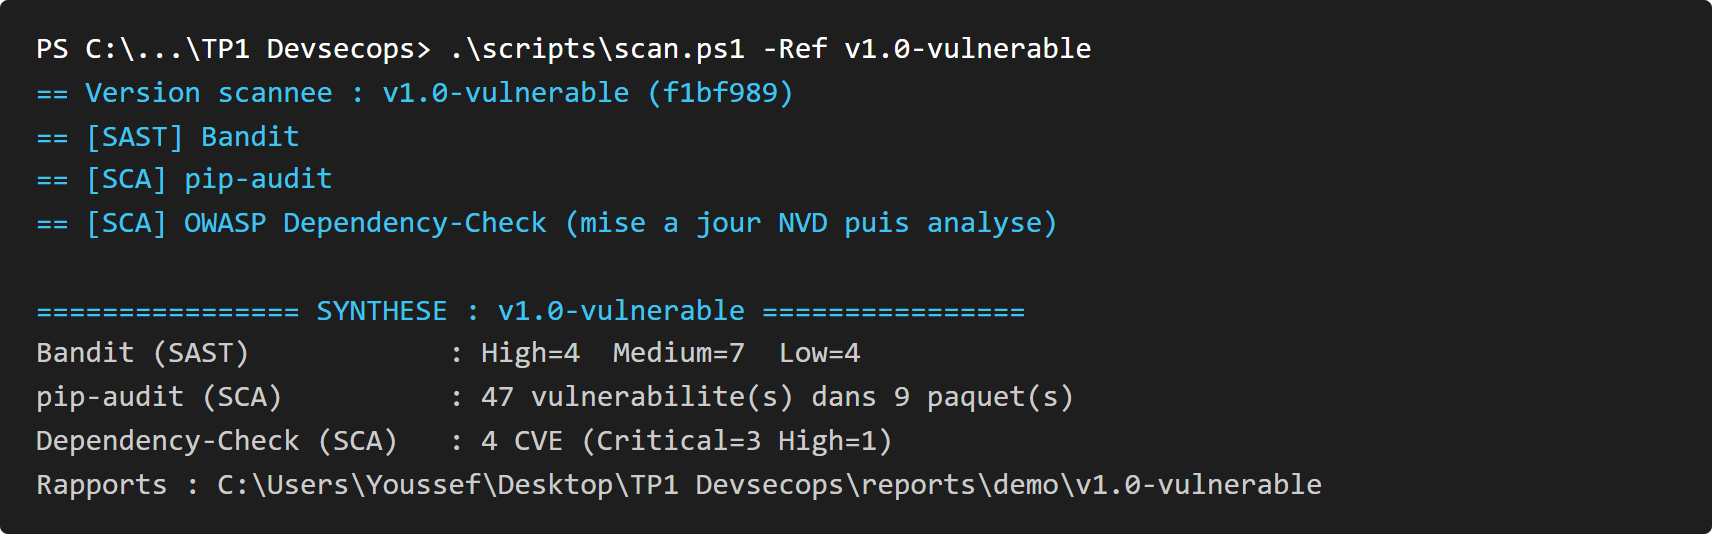
\includegraphics[width=0.92\textwidth]{t_scan_before.png}}
\caption{Script de démonstration sur la version initiale \code{v1.0-vulnerable}.}
\label{fig:scanbefore}
\end{figure}

\begin{figure}[H]
\centering
\fbox{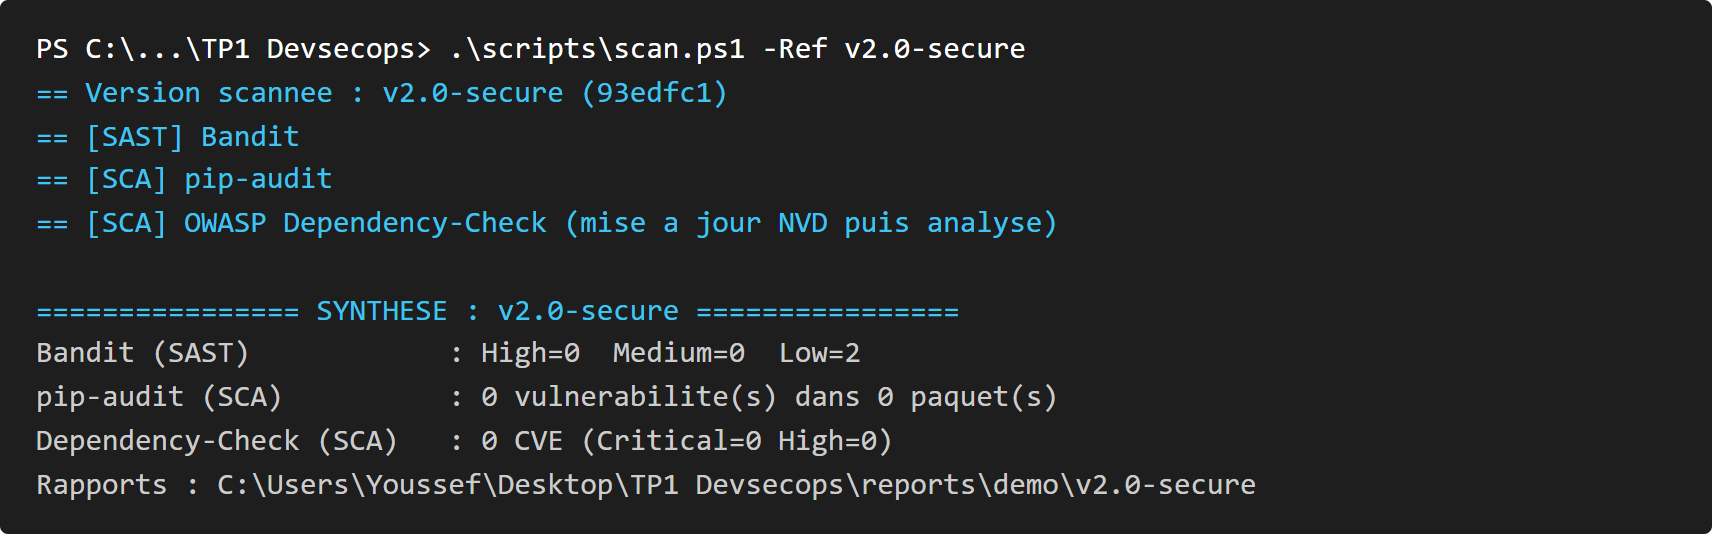
\includegraphics[width=0.92\textwidth]{t_scan_after.png}}
\caption{Script de démonstration sur la version corrigée \code{v2.0-secure}.}
\label{fig:scanafter}
\end{figure}

\begin{figure}[H]
\centering
\fbox{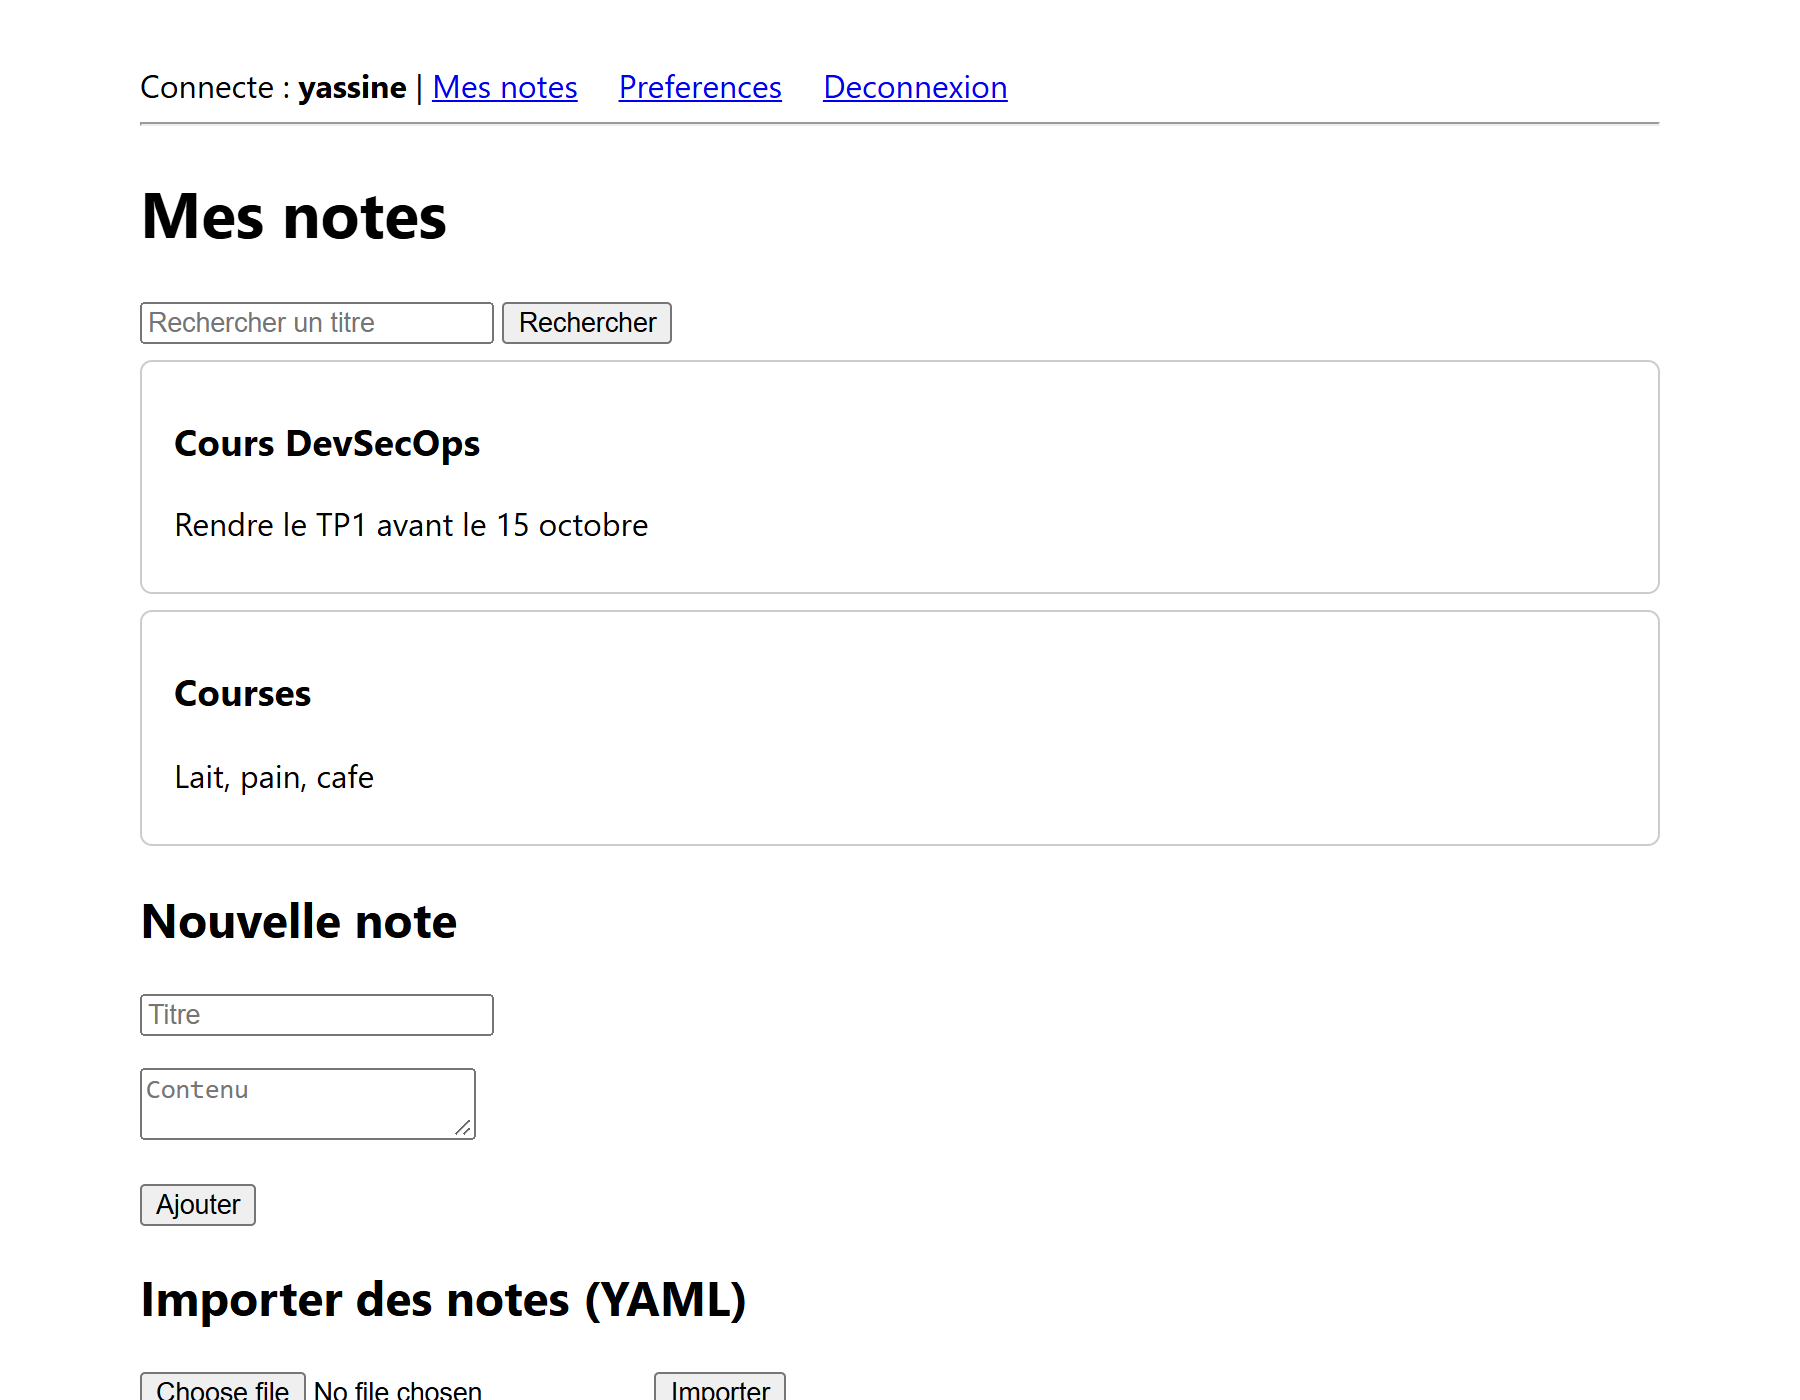
\includegraphics[width=0.7\textwidth]{a_secure_notes.png}}
\caption{Application corrigée (\code{http://localhost:5002}) : connexion et notes.}
\label{fig:notes}
\end{figure}

\begin{figure}[H]
\centering
\fbox{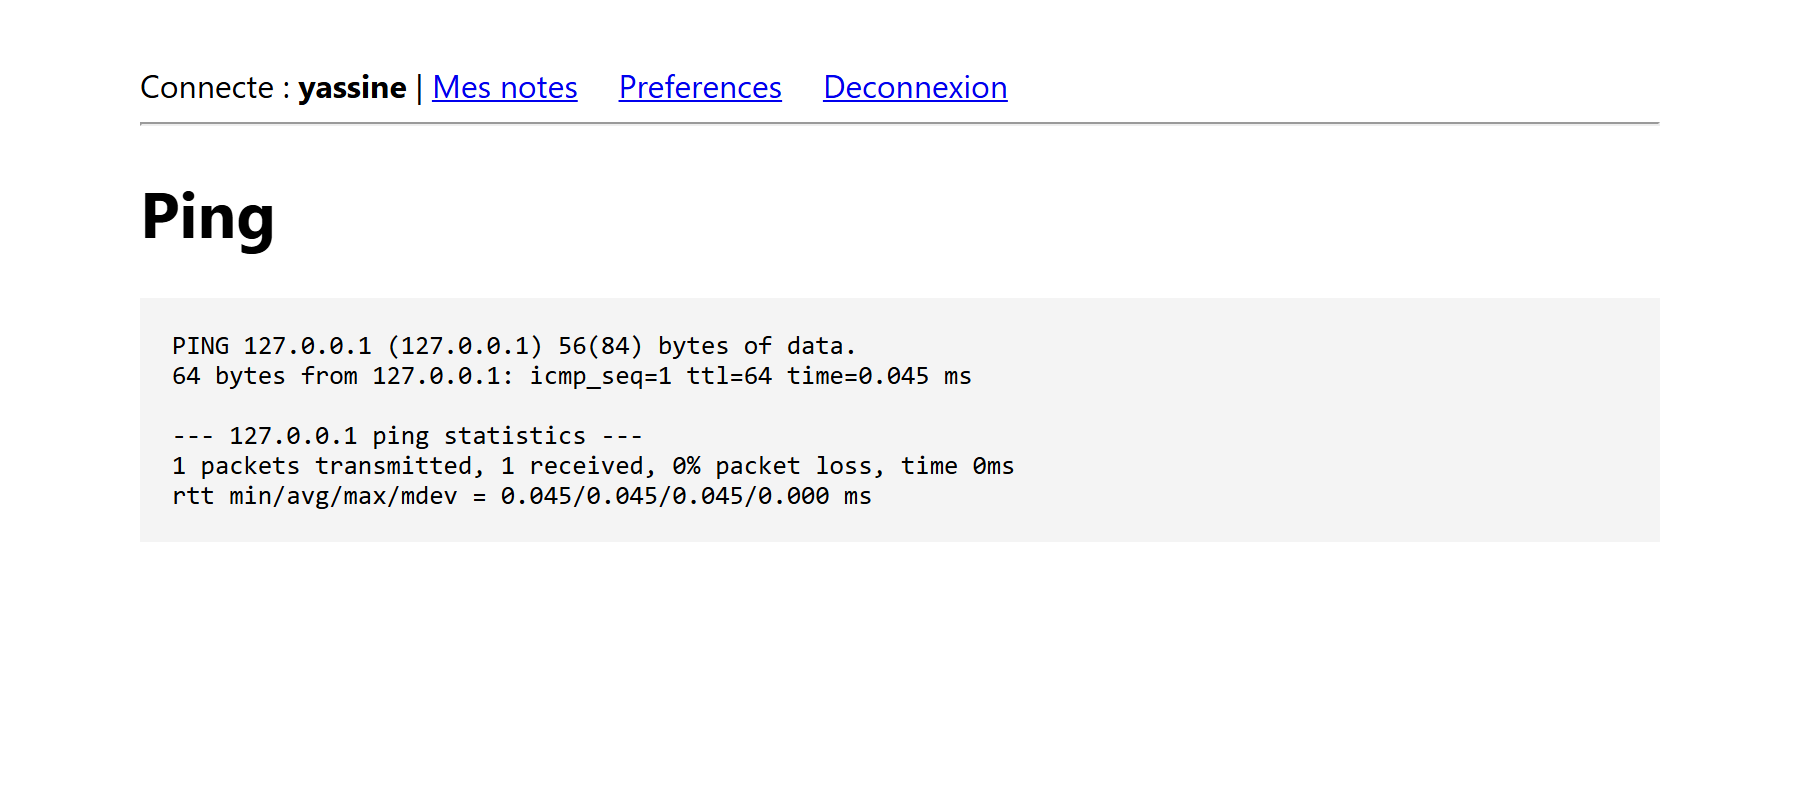
\includegraphics[width=0.7\textwidth]{a_secure_ping_ok.png}}
\caption{Outil ping avec une adresse IP valide.}
\label{fig:pingok}
\end{figure}

\begin{table}[H]
\centering
\begin{tabular}{@{}lcc@{}}
\toprule
 & \textbf{\code{v1.0-vulnerable}} & \textbf{\code{v2.0-secure}} \\
\midrule
Bandit -- High / Medium / Low & 4 / 7 / 4 & \textbf{0 / 0} / 2 \\
pip-audit & 47 (9 paquets) & \textbf{0} \\
Dependency-Check -- projet & 4 CVE (3 Critical) & \textbf{0} \\
Dependency-Check -- image & 44 alertes (7 Critical) & \textbf{0} \\
Image de base & Python 3.7 (EOL), root & Python 3.13, non-root \\
\bottomrule
\end{tabular}
\caption{Bilan avant / après}
\end{table}

\subsection{Automatisation dans le pipeline CI (shift-left)}
Le workflow \code{.github/}\allowbreak\code{workflows/security.yml} lance automatiquement les contrôles à chaque
\code{push} et \code{pull request} :

\begin{table}[H]
\centering
\begin{tabularx}{\textwidth}{@{}lL@{}}
\toprule
\textbf{Job} & \textbf{Condition d'échec} \\
\midrule
SAST -- Bandit & Un problème de sévérité $\geq$ Medium \\
SCA -- pip-audit & Une vulnérabilité connue dans \code{requirements.txt} \\
SCA -- OWASP Dependency-Check & Une CVE de score CVSS $\geq$ 7 (\code{-{}-failOnCVSS 7}) \\
Build Docker & L'image ne se construit pas \\
\bottomrule
\end{tabularx}
\end{table}

\noindent Ces contrôles jouent le rôle d'une \textbf{porte de qualité} (\emph{quality gate}). Une
modification qui réintroduirait \code{shell=True} ou une version vulnérable de PyYAML serait
bloquée avant d'être fusionnée (Figure~\ref{fig:gate}). Sur la version corrigée, les quatre jobs
réussissent (Figure~\ref{fig:ghrun}).


\begin{figure}[H]
\centering
\fbox{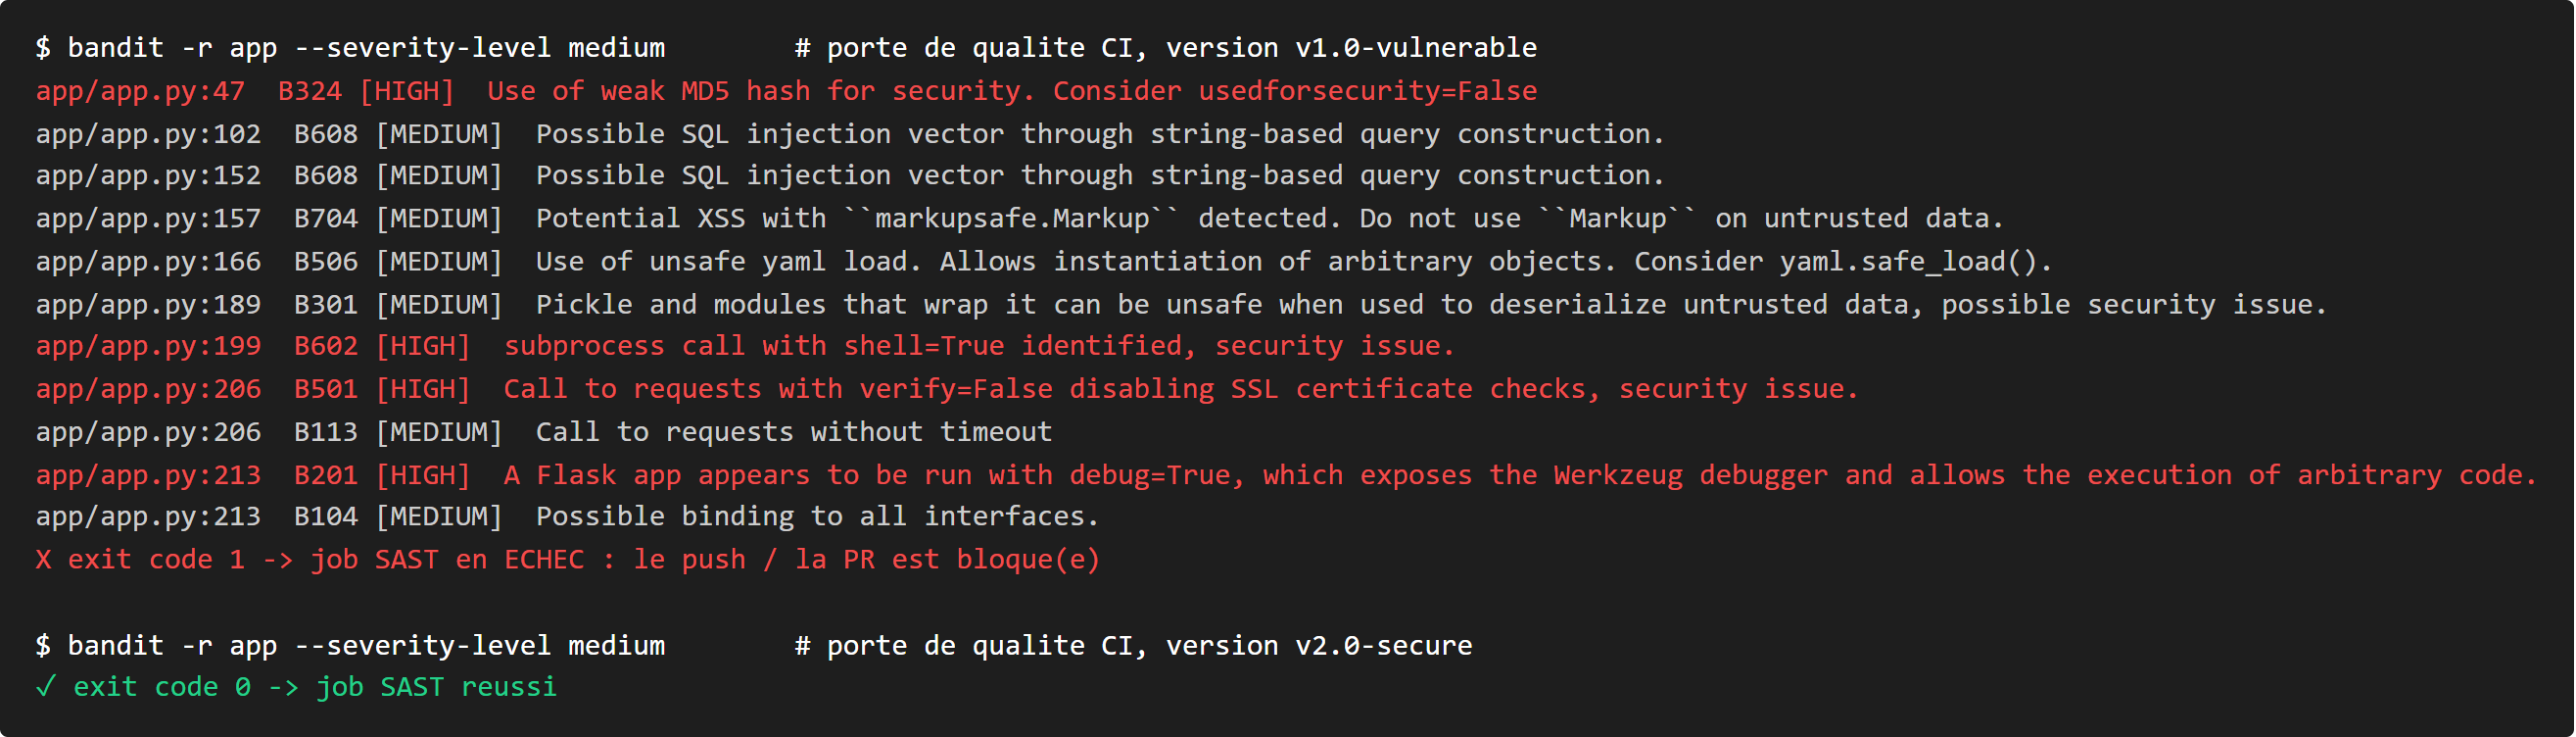
\includegraphics[width=0.98\textwidth]{t_gate.png}}
\caption{Porte de qualité SAST de la CI : échec sur la version initiale, succès sur la version corrigée.}
\label{fig:gate}
\end{figure}

\begin{figure}[H]
\centering
\fbox{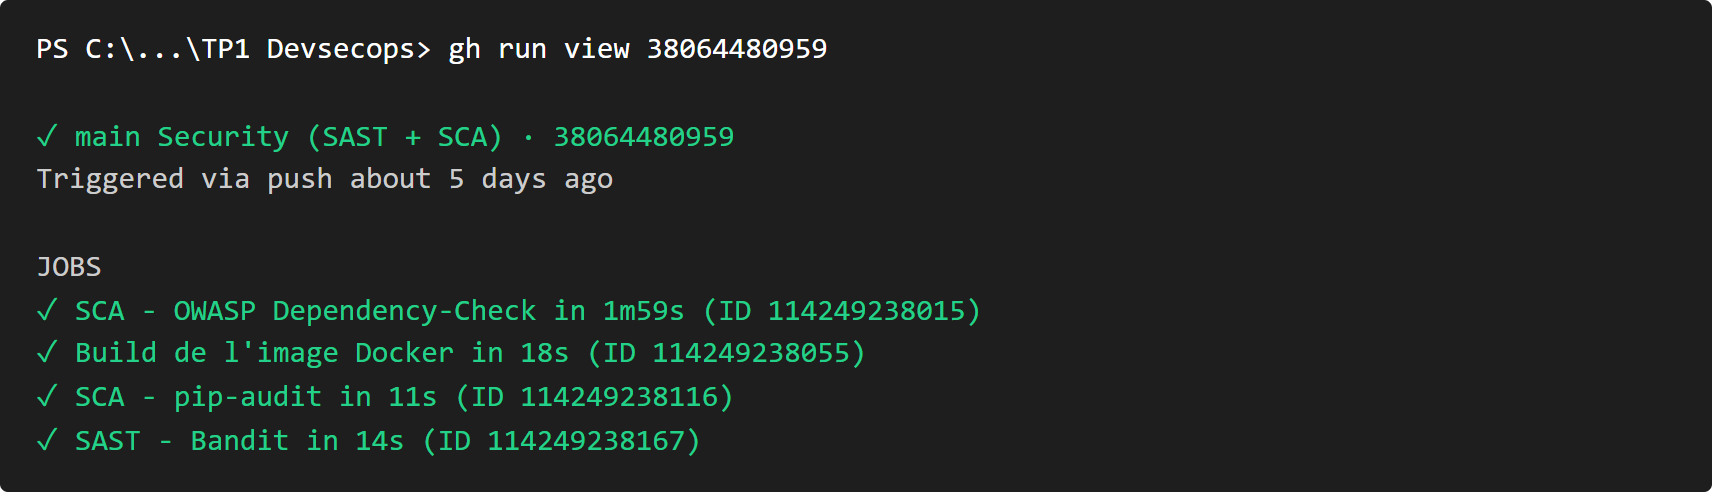
\includegraphics[width=0.92\textwidth]{t_gh_run.png}}
\caption{Exécution GitHub Actions réussie du pipeline \og Security (SAST + SCA) \fg.}
\label{fig:ghrun}
\end{figure}

% ---------------------------------------------------------------------------
\section{Conclusion}
% ---------------------------------------------------------------------------
Ce TP a permis d'appliquer concrètement l'approche shift-left sur une application web
conteneurisée. L'analyse \textbf{SAST} avec Bandit a révélé 15 problèmes, dont 11 de sévérité High
ou Medium, tous corrigés : injection SQL, injection de commande, XSS, désérialisation non sûre,
hachage faible, secrets en dur, mode debug\ldots{} L'analyse \textbf{SCA} a montré que la majorité
des vulnérabilités venait en réalité du code des autres : 47 vulnérabilités connues dans 9
dépendances, dont plusieurs critiques, toutes éliminées par la mise à jour des bibliothèques et de
l'image de base.

Le TP met aussi en évidence que SAST et SCA se renforcent mutuellement (\code{yaml.load} avec
PyYAML 5.3, \code{debug=True} avec Werkzeug 0.14), et qu'aucun outil n'est exhaustif : il faut
croiser les sources et trier les résultats. Enfin, l'intégration de ces scans dans un pipeline CI
transforme ces contrôles ponctuels en une protection continue.

\paragraph{Pistes d'amélioration.} Protection CSRF (Flask-WTF), \code{requirements.txt} avec
empreintes (\code{pip-compile -{}-generate-hashes}), mises à jour automatiques (Dependabot),
scan complet de l'image (Trivy), détection de secrets dans l'historique (gitleaks) et tests
dynamiques (DAST, OWASP ZAP).

% ---------------------------------------------------------------------------
\bigskip
\section*{Annexe -- Détail des vulnérabilités des dépendances}\label{sec:cve}
\addcontentsline{toc}{section}{Annexe -- Détail des vulnérabilités des dépendances}
% ---------------------------------------------------------------------------
Source : pip-audit (identifiants et versions corrigées), croisé avec Dependency-Check (scores
CVSS de la NVD). Un tiret indique que Dependency-Check n'a pas détecté la vulnérabilité.

{\footnotesize\setlength{\tabcolsep}{4pt}
\begin{longtable}{@{}lllllll@{}}
\toprule
\textbf{Paquet} & \textbf{Version} & \textbf{Identifiant} & \textbf{CVE} & \textbf{CVSS} & \textbf{Corrigé en} & \textbf{Retenue} \\
\midrule
\endhead
flask & 0.12.2 & PYSEC-2019-179 & CVE-2019-1010083 & -- & 1.0 & 3.1.3 \\
flask & 0.12.2 & PYSEC-2018-66 & CVE-2018-1000656 & -- & 0.12.3 & 3.1.3 \\
flask & 0.12.2 & PYSEC-2023-62 & CVE-2023-30861 & -- & 2.2.5 / 2.3.2 & 3.1.3 \\
flask & 0.12.2 & PYSEC-2026-2151 & CVE-2026-27205 & -- & 3.1.3 & 3.1.3 \\
werkzeug & 0.14.1 & PYSEC-2019-140 & CVE-2019-14806 & 7.5 High & 0.15.3 & 3.1.9 \\
werkzeug & 0.14.1 & PYSEC-2022-203 & CVE-2022-29361 & 9.8 Critical & 2.1.1 & 3.1.9 \\
werkzeug & 0.14.1 & PYSEC-2026-1065 & CVE-2019-14322 & 7.5 High & 0.15.5 & 3.1.9 \\
werkzeug & 0.14.1 & PYSEC-2023-57 & CVE-2023-23934 & 3.5 Low & 2.2.3 & 3.1.9 \\
werkzeug & 0.14.1 & PYSEC-2023-58 & CVE-2023-25577 & 7.5 High & 2.2.3 & 3.1.9 \\
werkzeug & 0.14.1 & PYSEC-2023-221 & CVE-2023-46136 & 7.5 High & 2.3.8 / 3.0.1 & 3.1.9 \\
werkzeug & 0.14.1 & PYSEC-2026-2043 & CVE-2024-34069 & 7.5 High & 3.0.3 & 3.1.9 \\
werkzeug & 0.14.1 & PYSEC-2026-2045 & CVE-2024-49766 & 5.3 Medium & 3.0.6 & 3.1.9 \\
werkzeug & 0.14.1 & PYSEC-2026-2046 & CVE-2025-66221 & 5.3 Medium & 3.1.4 & 3.1.9 \\
werkzeug & 0.14.1 & PYSEC-2026-2044 & CVE-2026-21860 & 5.3 Medium & 3.1.5 & 3.1.9 \\
werkzeug & 0.14.1 & PYSEC-2026-2320 & CVE-2026-27199 & 5.3 Medium & 3.1.6 & 3.1.9 \\
werkzeug & 0.14.1 & CVE-2026-102598 & CVE-2026-102598 & -- & 3.1.9 & 3.1.9 \\
jinja2 & 2.10 & PYSEC-2021-66 & CVE-2020-28493 & -- & 2.11.3 & 3.1.6 \\
jinja2 & 2.10 & PYSEC-2019-217 & CVE-2019-10906 & -- & 2.10.1 & 3.1.6 \\
jinja2 & 2.10 & PYSEC-2026-1473 & CVE-2024-22195 & -- & 3.1.3 & 3.1.6 \\
jinja2 & 2.10 & PYSEC-2026-1474 & CVE-2024-34064 & -- & 3.1.4 & 3.1.6 \\
jinja2 & 2.10 & PYSEC-2026-1475 & CVE-2024-56326 & -- & 3.1.5 & 3.1.6 \\
jinja2 & 2.10 & PYSEC-2026-1471 & CVE-2025-27516 & -- & 3.1.6 & 3.1.6 \\
pyyaml & 5.3 & PYSEC-2020-96 & CVE-2020-1747 & 9.8 Critical & 5.3.1 & 6.0.3 \\
pyyaml & 5.3 & PYSEC-2021-142 & CVE-2020-14343 & 9.8 Critical & 5.4 & 6.0.3 \\
requests & 2.19.1 & PYSEC-2018-28 & CVE-2018-18074 & 7.5 High & 2.20.0 & 2.34.2 \\
requests & 2.19.1 & PYSEC-2023-74 & CVE-2023-32681 & 6.1 Medium & 2.31.0 & 2.34.2 \\
requests & 2.19.1 & PYSEC-2026-1873 & CVE-2024-35195 & -- & 2.32.0 & 2.34.2 \\
requests & 2.19.1 & PYSEC-2026-1872 & CVE-2024-47081 & -- & 2.32.4 & 2.34.2 \\
requests & 2.19.1 & PYSEC-2026-2275 & CVE-2026-25645 & 5.5 Medium & 2.33.0 & 2.34.2 \\
urllib3 & 1.23 & PYSEC-2019-133 & CVE-2019-11324 & -- & 1.24.2 & 2.8.0 \\
urllib3 & 1.23 & PYSEC-2019-132 & CVE-2019-11236 & -- & 1.24.3 & 2.8.0 \\
urllib3 & 1.23 & PYSEC-2020-148 & CVE-2020-26137 & -- & 1.25.9 & 2.8.0 \\
urllib3 & 1.23 & PYSEC-2026-1995 & CVE-2024-37891 & -- & 1.26.19 / 2.2.2 & 2.8.0 \\
urllib3 & 1.23 & PYSEC-2023-192 & CVE-2023-43804 & -- & 1.26.17 / 2.0.6 & 2.8.0 \\
urllib3 & 1.23 & PYSEC-2023-207 & CVE-2018-25091 & -- & 1.24.2 & 2.8.0 \\
urllib3 & 1.23 & PYSEC-2023-212 & CVE-2023-45803 & -- & 1.26.18 / 2.0.7 & 2.8.0 \\
urllib3 & 1.23 & PYSEC-2026-1999 & CVE-2025-50181 & -- & 2.5.0 & 2.8.0 \\
urllib3 & 1.23 & PYSEC-2026-1994 & CVE-2025-66471 & -- & 2.6.0 & 2.8.0 \\
urllib3 & 1.23 & PYSEC-2026-1996 & CVE-2026-21441 & -- & 2.6.3 & 2.8.0 \\
urllib3 & 1.23 & PYSEC-2026-141 & CVE-2026-44431 & -- & 2.7.0 & 2.8.0 \\
urllib3 & 1.23 & PYSEC-2026-4177 & CVE-2026-97689 & -- & 2.8.0 & 2.8.0 \\
idna & 2.7 & PYSEC-2024-60 & CVE-2024-3651 & -- & 3.7 & 3.20 \\
idna & 2.7 & PYSEC-2026-215 & CVE-2026-45409 & -- & 3.15 & 3.20 \\
certifi & 2018.4.16 & PYSEC-2022-42986 & CVE-2022-23491 & 7.5 High & 2022.12.7 & 2026.7.22 \\
certifi & 2018.4.16 & PYSEC-2023-135 & CVE-2023-37920 & 9.8 Critical & 2023.7.22 & 2026.7.22 \\
gunicorn & 19.9.0 & PYSEC-2026-1434 & CVE-2024-1135 & -- & 22.0.0 & 26.2.0 \\
gunicorn & 19.9.0 & PYSEC-2026-1433 & CVE-2024-6827 & -- & 22.0.0 & 26.2.0 \\
\bottomrule
\end{longtable}
}

\end{document}
